\chapter{Literature Review}

The landscape of calendar management and scheduling applications has evolved significantly with technological advancement and changing user needs. This chapter presents a comprehensive analysis of existing solutions, market research, and technological foundations that inform Jadwal's development. Through examining current tools, academic research, and user behavior patterns, we identify gaps in existing solutions and validate Jadwal's innovative approach to calendar management.

\section{Introduction}

In the modern world, managing time effectively is important for balancing personal and professional responsibilities.
The increasing complexity of schedules usually results in missing an important event and overlapping commitments.
To solve these challenges, we introduce Jadwal, an innovative iOS-based schedule management application, aims to help individuals and professionals to organize their daily lives.

Jadwal focuses on solving the issue by drawing inspiration from existing solutions like Clockwise, Motion, Reclaim AI, and Calendi, Jadwal stands out by introducing advance features such as conflict resolution, task prioritization, event extraction from informal communicating channels and prioritizing prayer times, which is a unique feature which is not found in any competing applications.

In developing Jadwal, we have drawn inspiration from and built upon existing research and products in the field of intelligent calendar management.
Some key references include:
\begin{itemize}
    \item \textbf{Clockwise (https://www.getclockwise.com/):} A smart calendar assistant that optimizes schedules and manages team coordination \cite{clockwise}. Clockwise's approach to intelligent time blocking and meeting optimization provides valuable insights for Jadwal's automated scheduling features.
    \item \textbf{Motion (https://www.usemotion.com/):} Motion's Intelligent Calendar takes your meetings, your tasks, your to-do list, your activities, and creates one perfect, optimized schedule to get it all done \cite{motion}.
    \item \textbf{Reclaim AI (https://reclaim.ai/):} An intelligent time management tool that helps optimize schedules and automate tasks \cite{reclaim}.
    \item \textbf{Calendi (https://calendi.ai/):} Calendi describes itself as: ``Calendi is an AI calendar system. Use it for scheduling tasks, automating meetings, and witness the future of calendar.'' \cite{calendi}
    \item \textbf{An Exploratory Study of Calendar Use:} ``Prospective remembering is the use of memory for remembering to do things in the future, as different from retrospective memory functions such as recalling past events.'' \cite{tungare2008exploratorystudycalendaruse}
    \item \textbf{WhatsApp Integration:} Our research indicates that direct WhatsApp integration for event extraction has not been widely implemented in existing calendar applications, making this a unique feature of Jadwal.
\end{itemize}

\begin{figure}[!h]
    \centering
    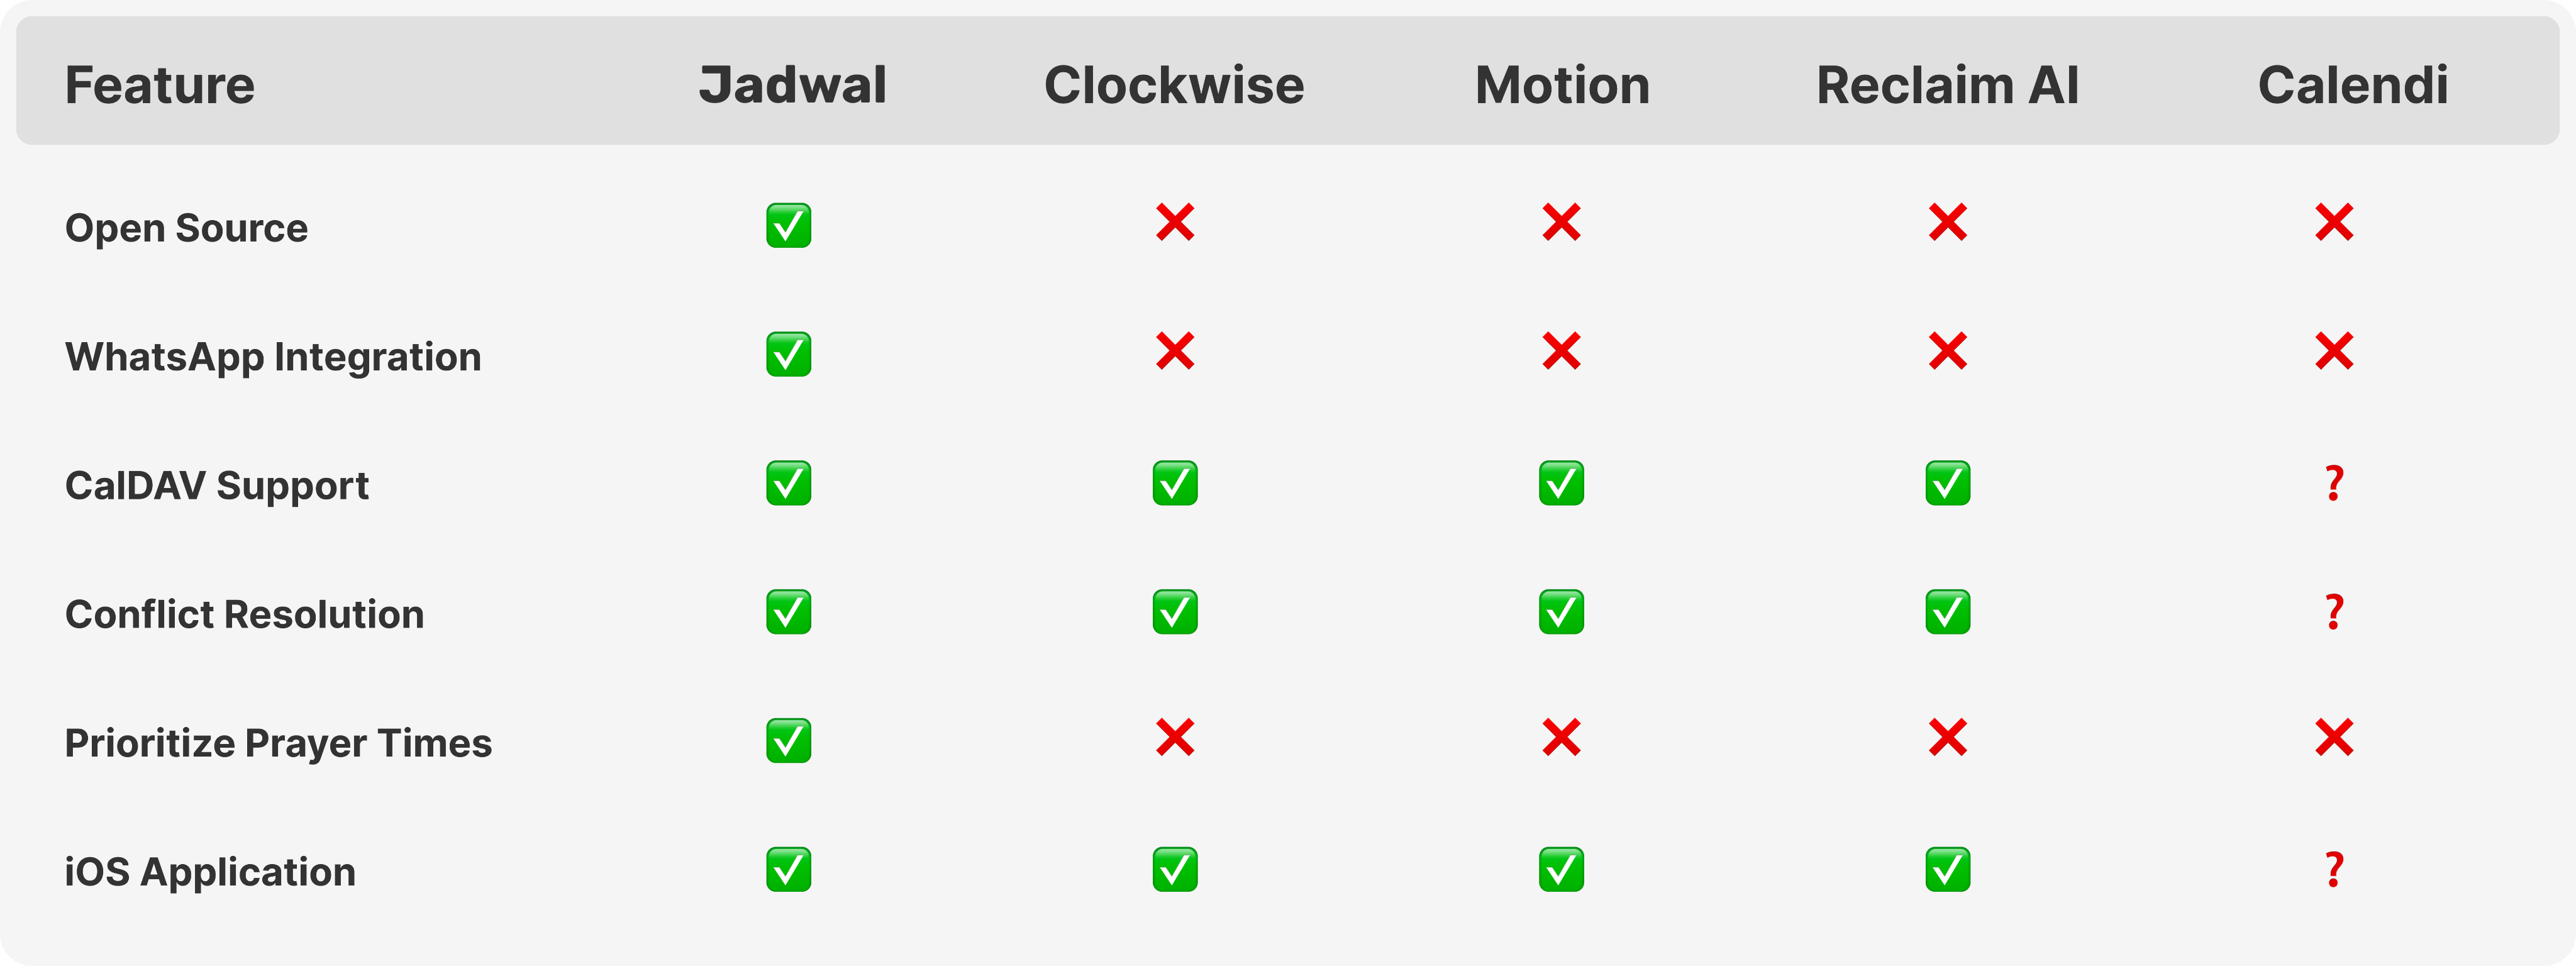
\includegraphics[width=\textwidth]{images/features-table.png}
    \caption{Feature Comparison Table}
    \label{fig:features-table}
\end{figure}



In Figure~\ref{fig:features-table} The table compares \textit{Jadwal}, our project, with four other scheduling applications—Clockwise, Motion, Reclaim AI, and Calendi—based based on several key features:
\begin{itemize}
    \item \textbf{Open Source}: \textit{Jadwal} stands out as the only application that is open-source, allowing users and developers to access, modify, and improve the code. The other applications do not provide this.
    \item \textbf{WhatsApp Integration}: \textit{Jadwal} stands out again as the only application that connects and extract the event discussed over the platform by the user.
    \item \textbf{CalDAV Support}: \textit{Jadwal}, Clockwise, and Reclaim AI offer CalDAV support, which allows users to integrate calendars from different sources, while Motion and Calendi either does not support this.
    \item \textbf{Conflict Resolution}: All listed applications, including \textit{Jadwal}, supports conflict resolution, allowing users to manage overlapping events efficiently.
    \item \textbf{Prioritize Prayer Times}: \textit{Jadwal} is the only one offering this feature where the user be able to have prayer time scheduled
    \item \textbf{iOS Application}: \textit{Jadwal} is available on iOS, along with Clockwise, Reclaim AI, and Motion. The availability of Calendi on iOS is uncertain.
\end{itemize}

\section{Comparing Competitors}

To thoroughly understand Jadwal's position in the market and its unique value proposition, a detailed analysis of existing calendar management solutions is essential. This section examines four major competitors—Clockwise, Motion, Reclaim AI, and Calendi—evaluating their features, strengths, and limitations to highlight how Jadwal addresses gaps in current offerings.

\subsection{Clockwise}

Clockwise's website tries to touch the user's misery by saying ``Your calendar doesn't have to suck'' as shown in Figure~\ref{fig:clockwise-landing}.

\begin{figure}[!h]
    \centering
    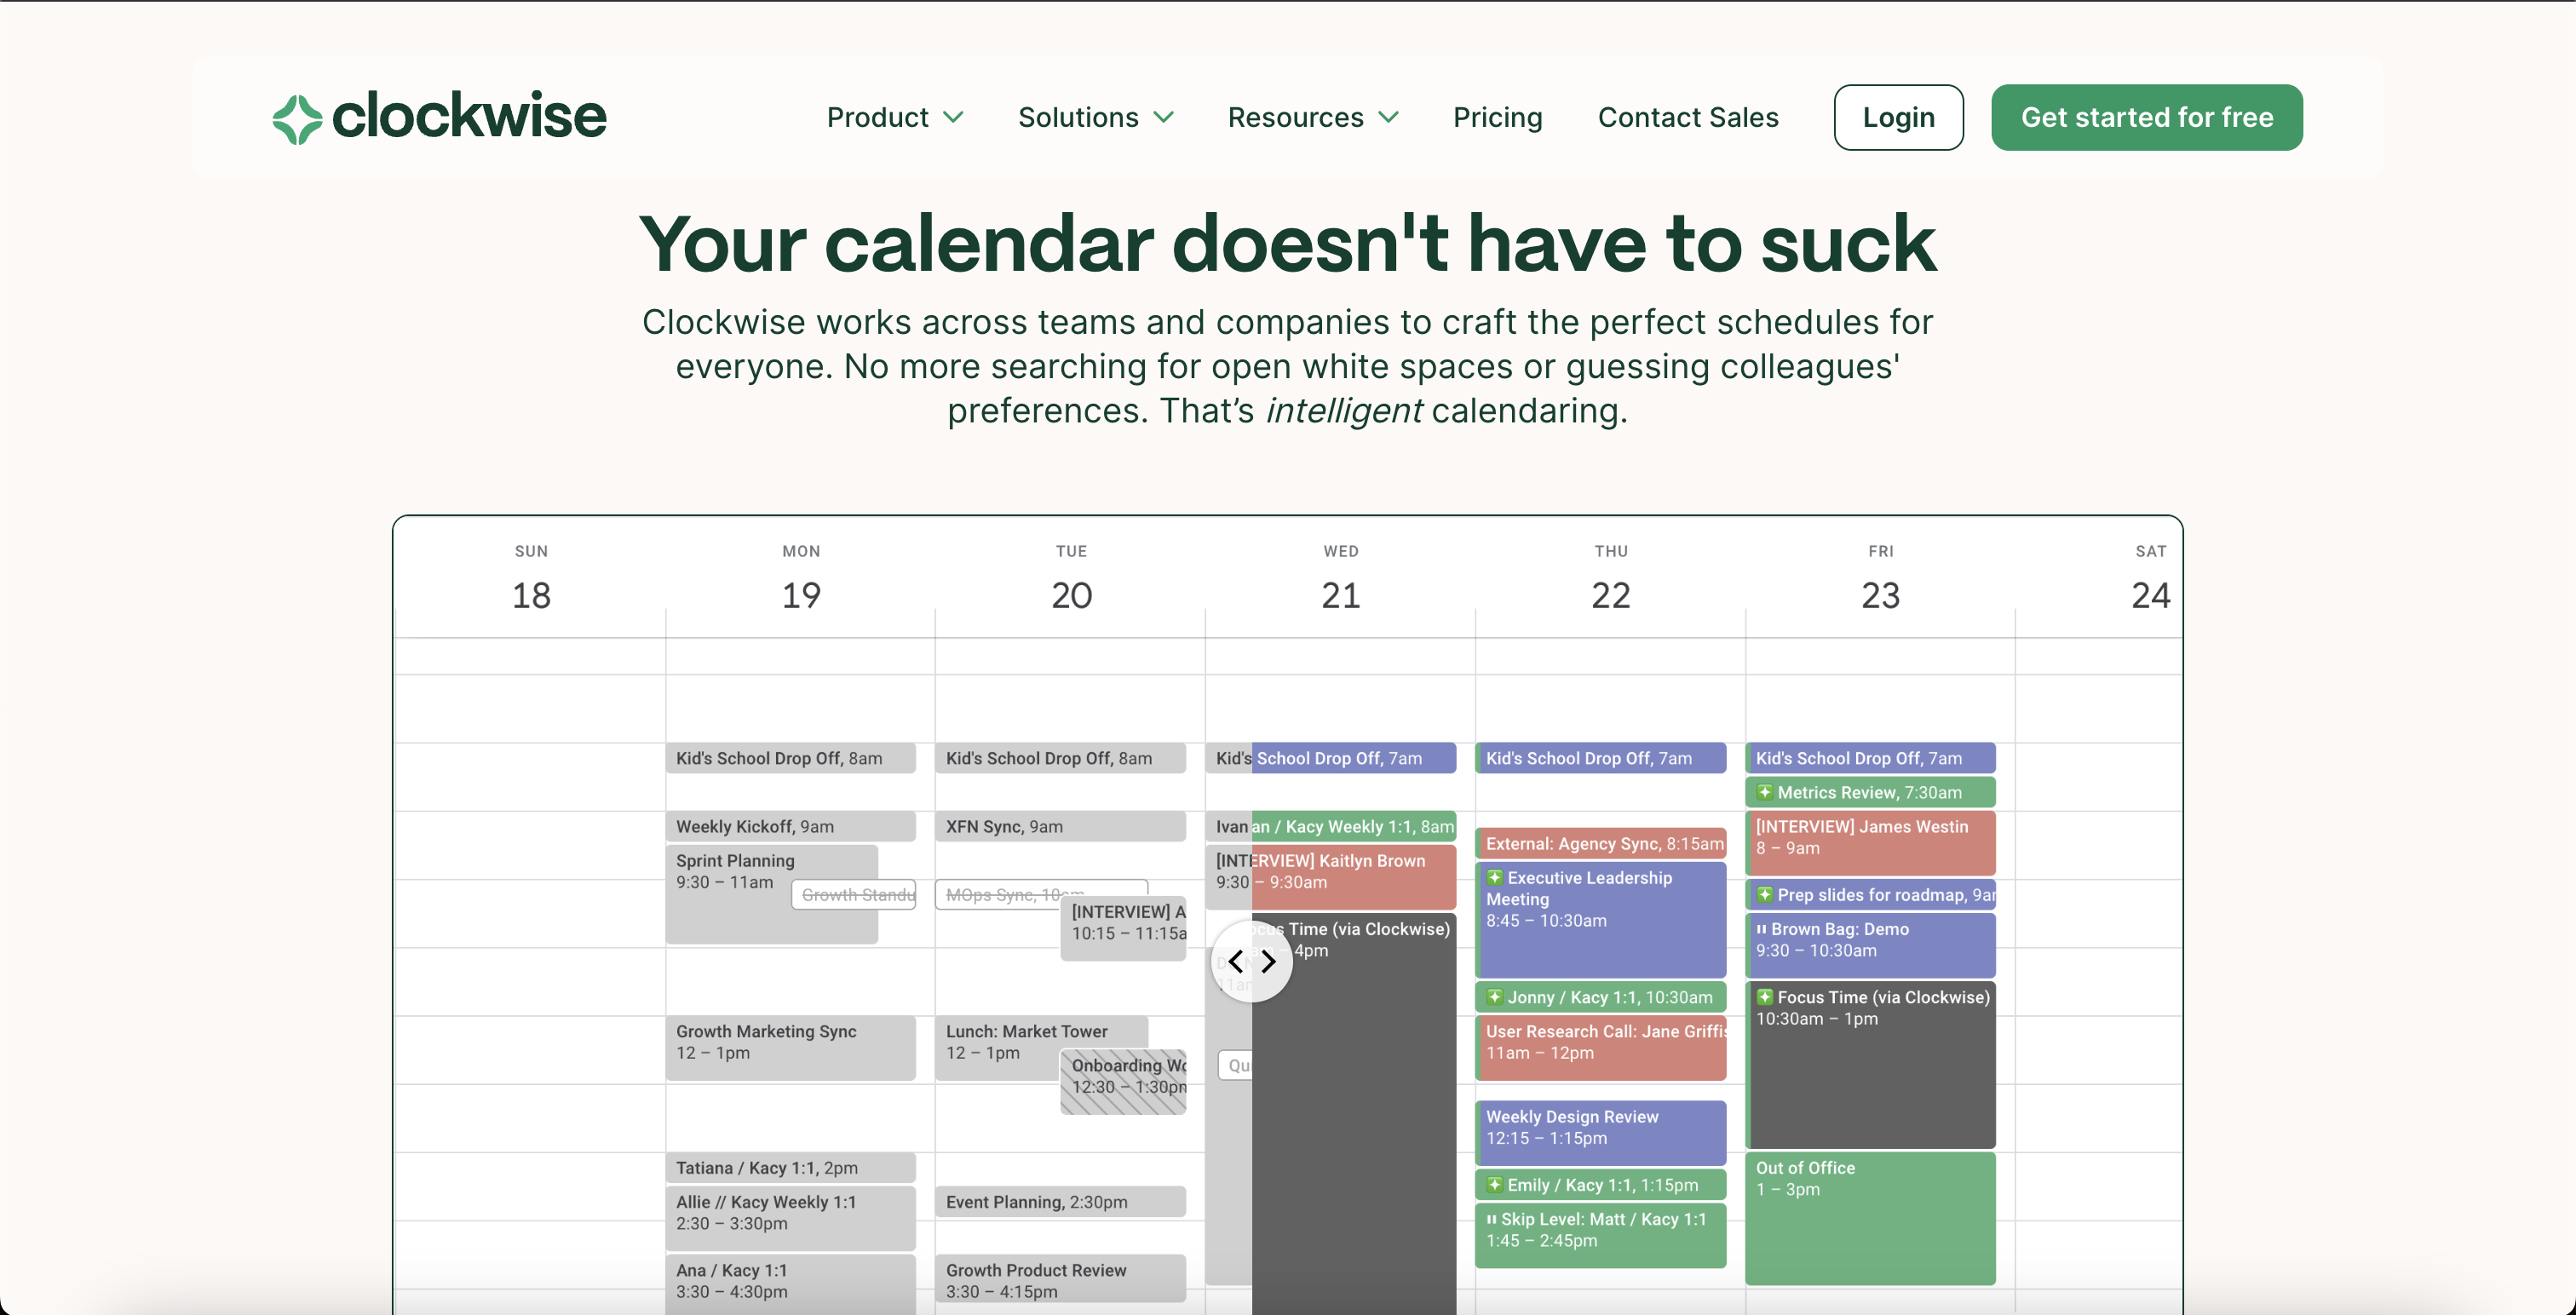
\includegraphics[width=0.8\textwidth]{images/competitors/clockwise-landing.png}
    \caption{Clockwise Landing Page}
    \label{fig:clockwise-landing}
\end{figure}

Based on Figure~\ref{fig:clockwise-features}, Clockwise has the following features:
\begin{itemize}
    \item Connect your calendar and set your preferences
    \item Decide which meetings are flexible
    \item Let Clockwise optimize your day
\end{itemize}

\begin{figure}[!h]
    \centering
    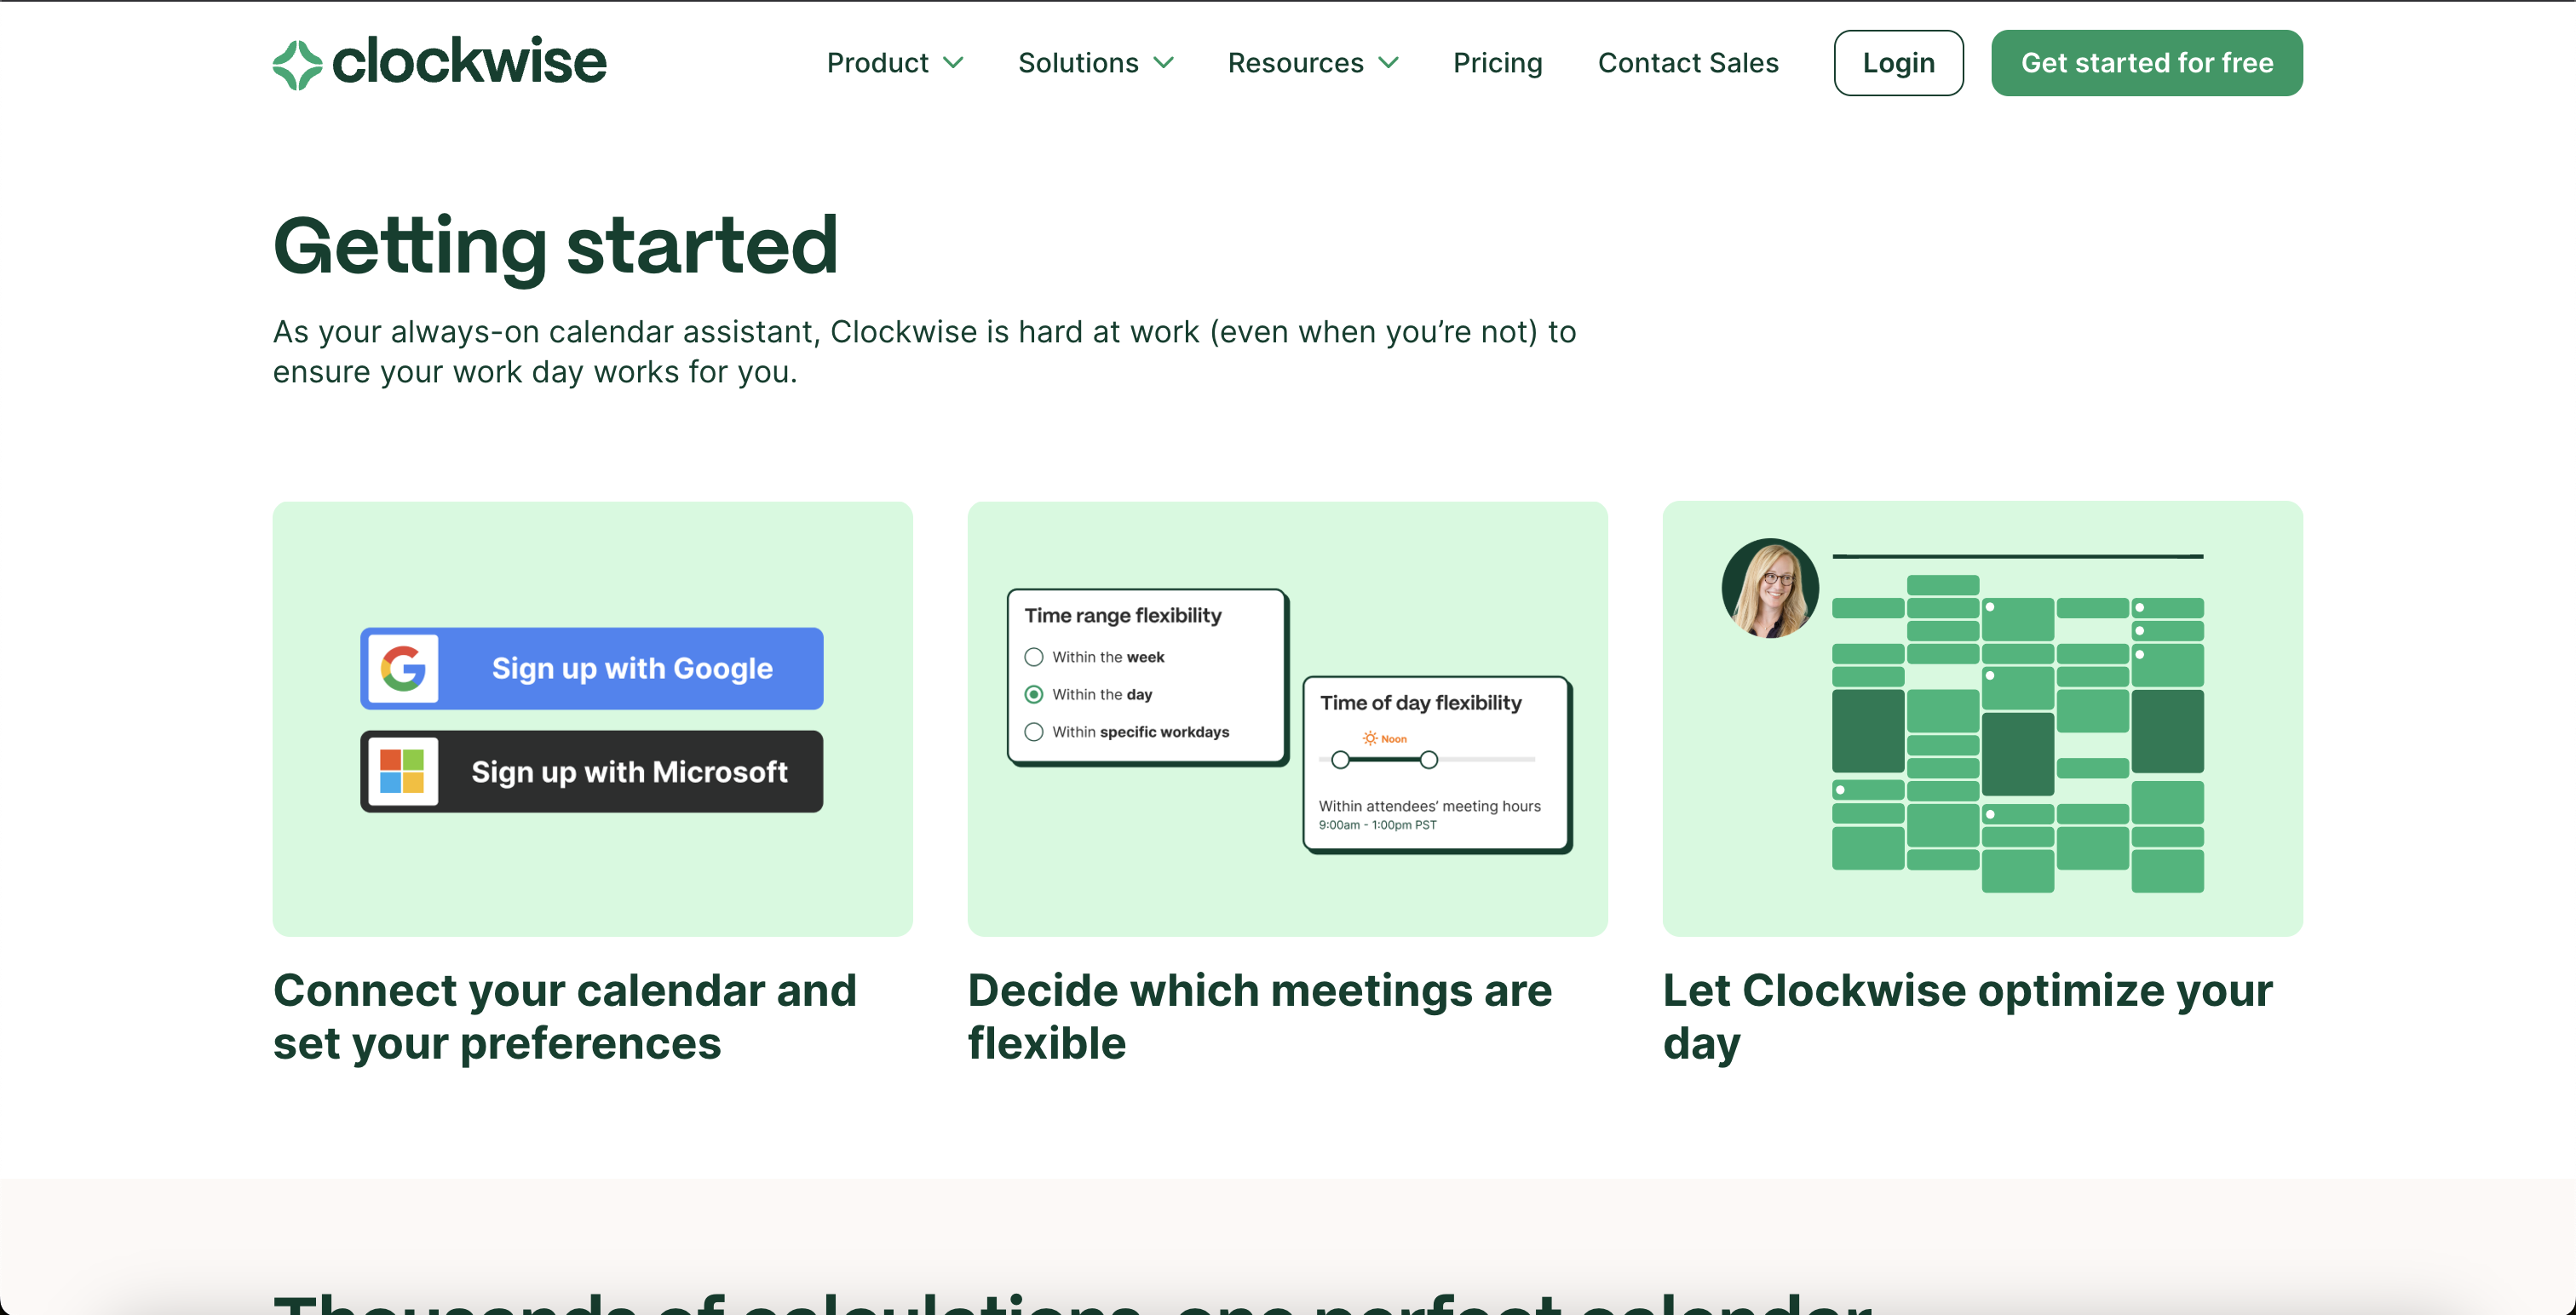
\includegraphics[width=0.8\textwidth]{images/competitors/clockwise-features.png}
    \caption{Clockwise Features Page}
    \label{fig:clockwise-features}
\end{figure}

\subsection{Motion}

Motion's website boasts about AI features in their landing page, as shown in Figure \ref{fig:motion-landing}.

\begin{figure}[!h]
    \centering
    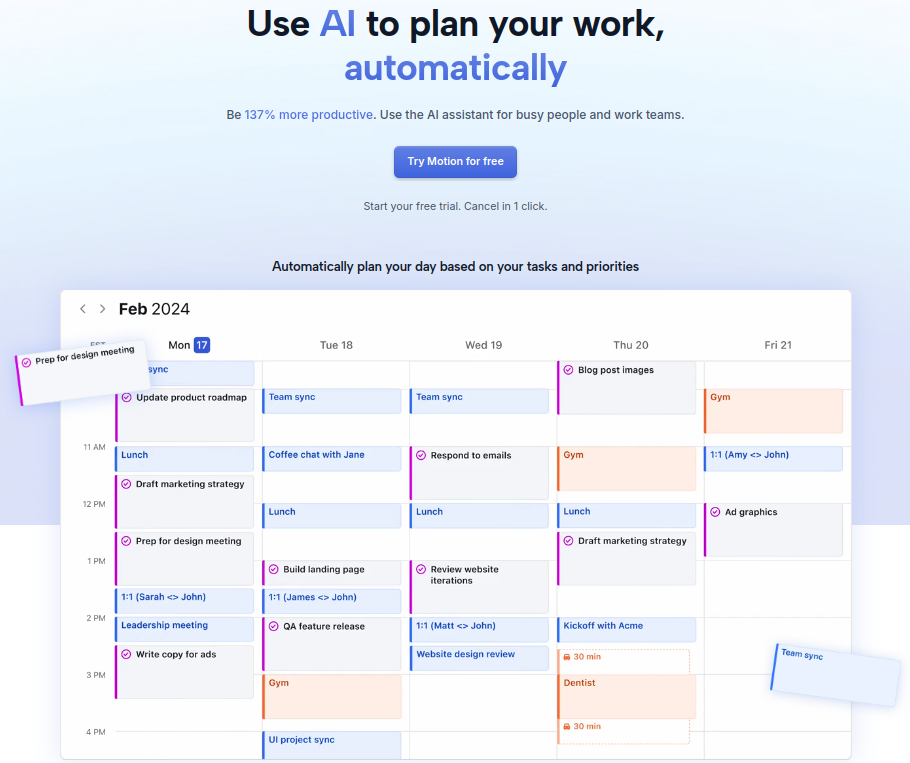
\includegraphics[width=0.8\textwidth]{images/competitors/motion-landing.png}
    \caption{Motion's Landing Page}
    \label{fig:motion-landing}
\end{figure}

Its features include a dynamic calendar that automatically prioritizes tasks, suggests optimized schedules, and helps users adapt to changes seamlessly.

The tool also provides team collaboration features, allowing shared schedules and streamlined task management to enhance team productivity.
These features ensure that users can achieve maximum efficiency with minimal effort.

Motion allows you to combine your calendars in one view also, shown in Figure~\ref{fig:motion-combined-calendar}.

\begin{figure}[!h]
    \centering
    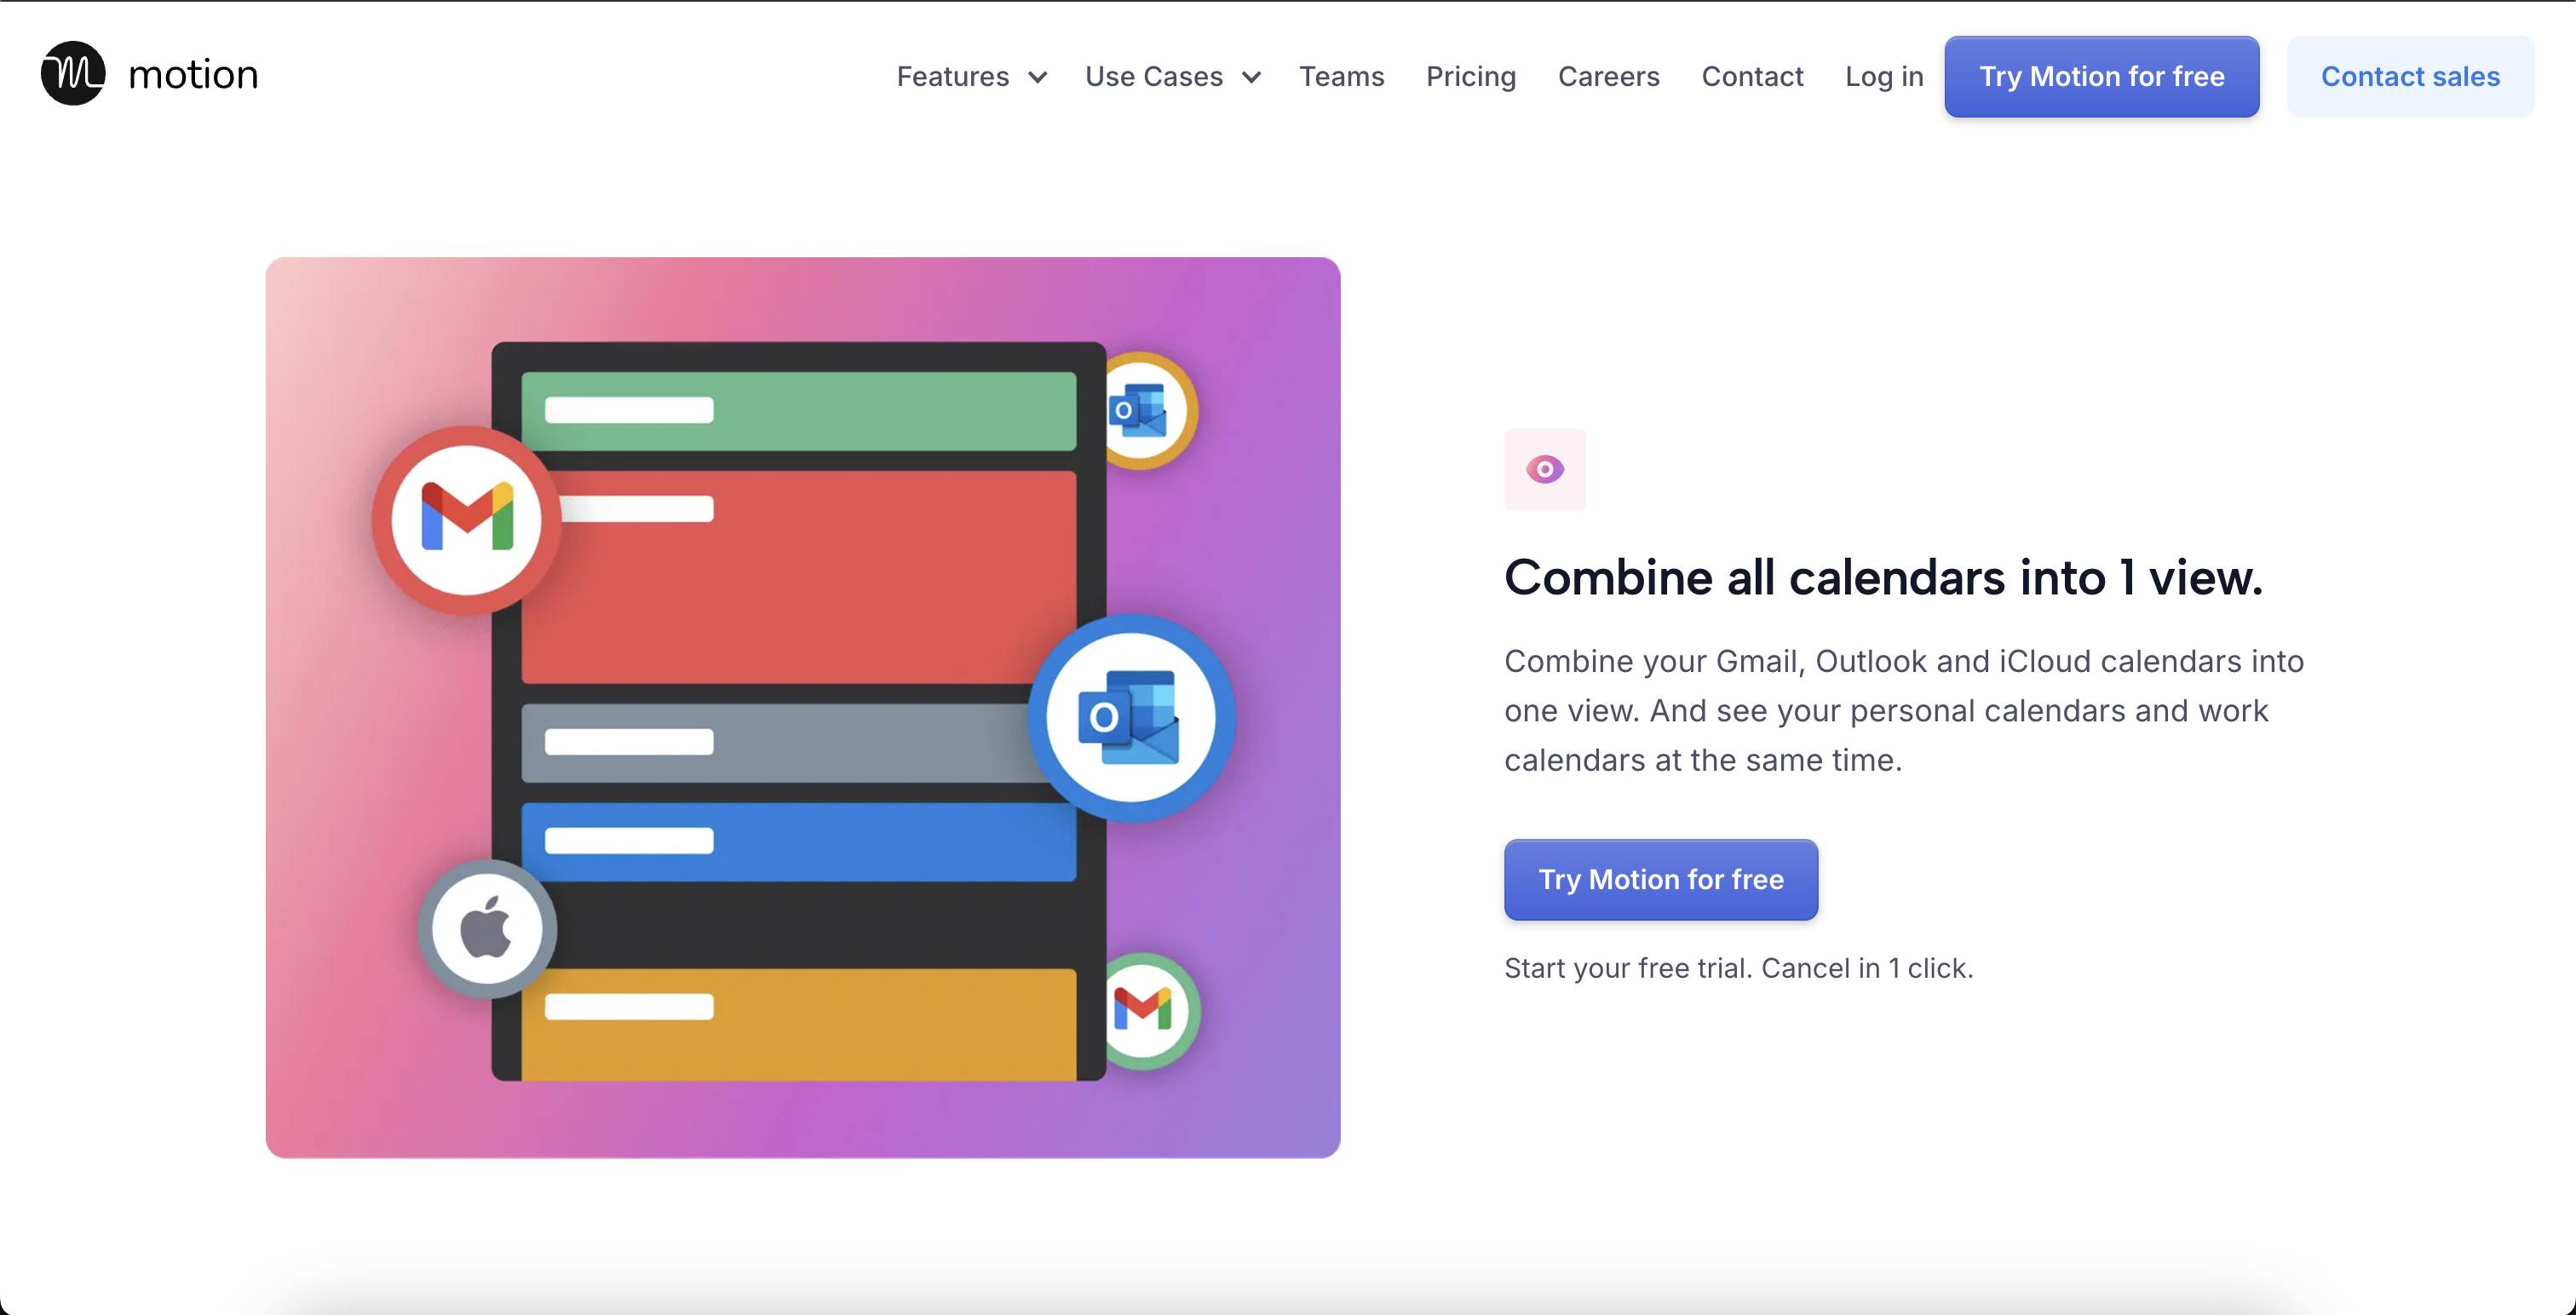
\includegraphics[width=0.8\textwidth]{images/competitors/motion-combined-calendar.png}
    \caption{Motion's Combined Calendar Feature}
    \label{fig:motion-combined-calendar}
\end{figure}

Motion also has a time blocking feature which they boast about in the website.
It is shown in Figure~\ref{fig:motion-time-blocking}.

\begin{figure}[!h]
    \centering
    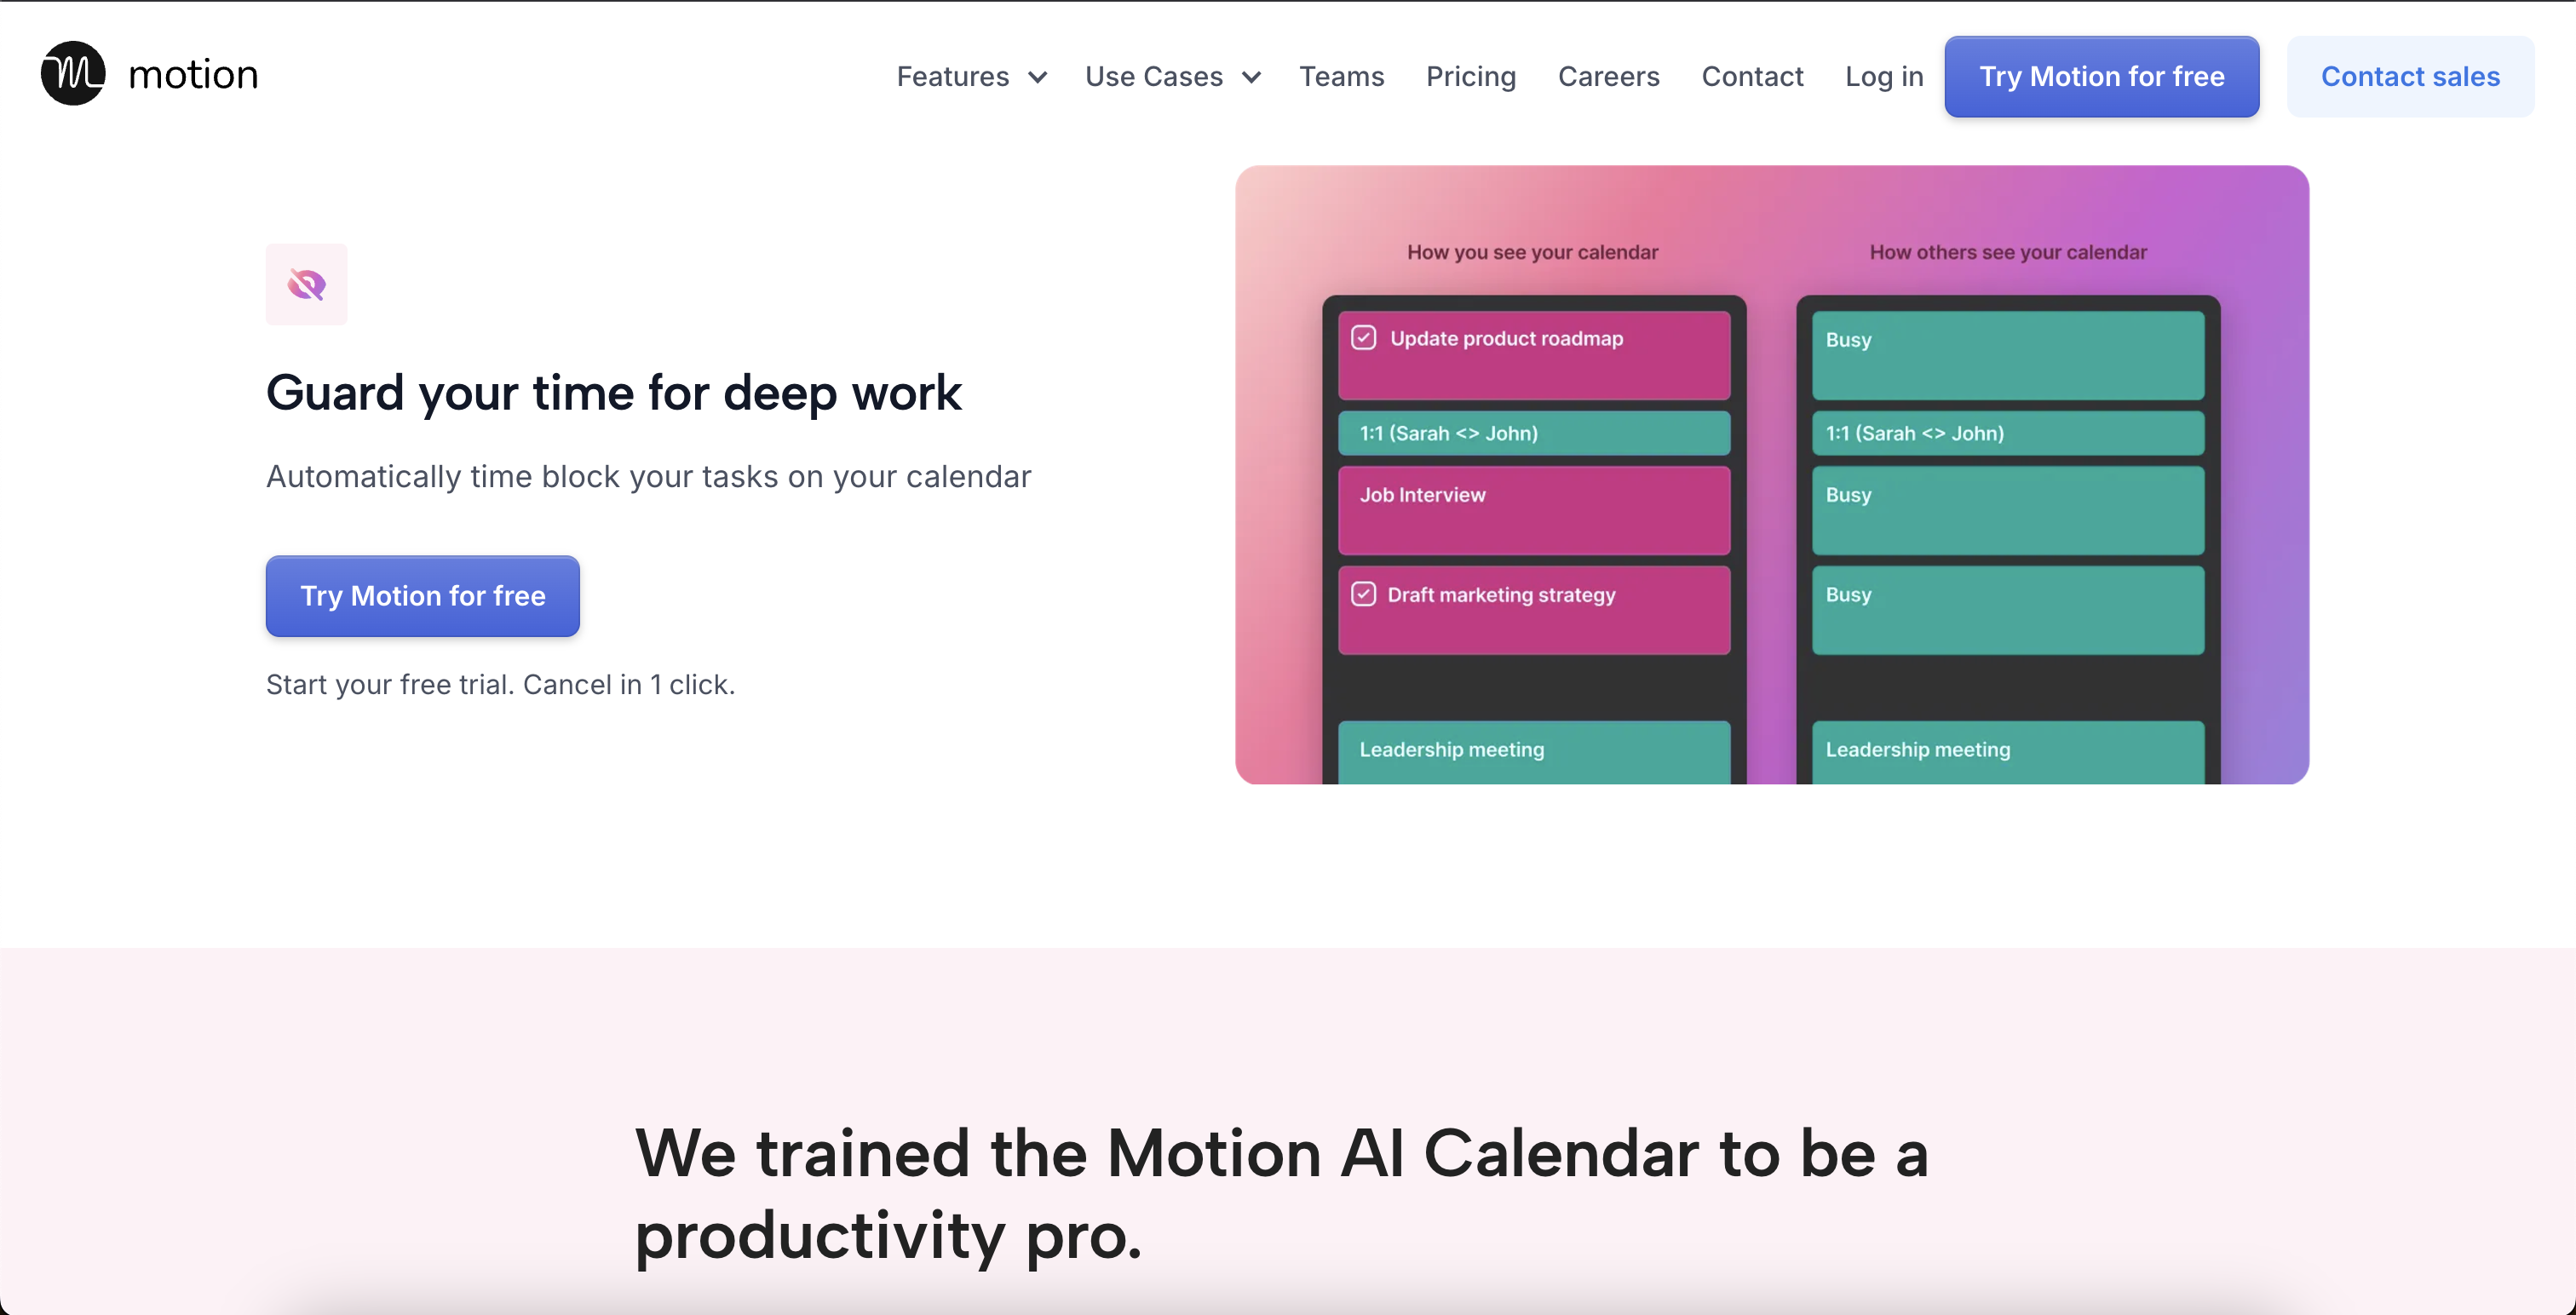
\includegraphics[width=0.8\textwidth]{images/competitors/motion-time-blocking.png}
    \caption{Motion's Time Blocking Feature}
    \label{fig:motion-time-blocking}
\end{figure}

Jadwal platform, such as linking the calendar to WhatsApp for automatic event addition and integrating prayer times, which adds a unique level of customization and day organization.

\subsection{Reclaim AI}

Reclaim.ai offers the following features: It is an AI-powered platform designed to manage tasks, habits, meetings, and personal events seamlessly.
Figure~\ref{fig:reclaim-landing} shows the the landing page of Reclaim and their focus on AI as you can see.

\begin{figure}[!h]
    \centering
    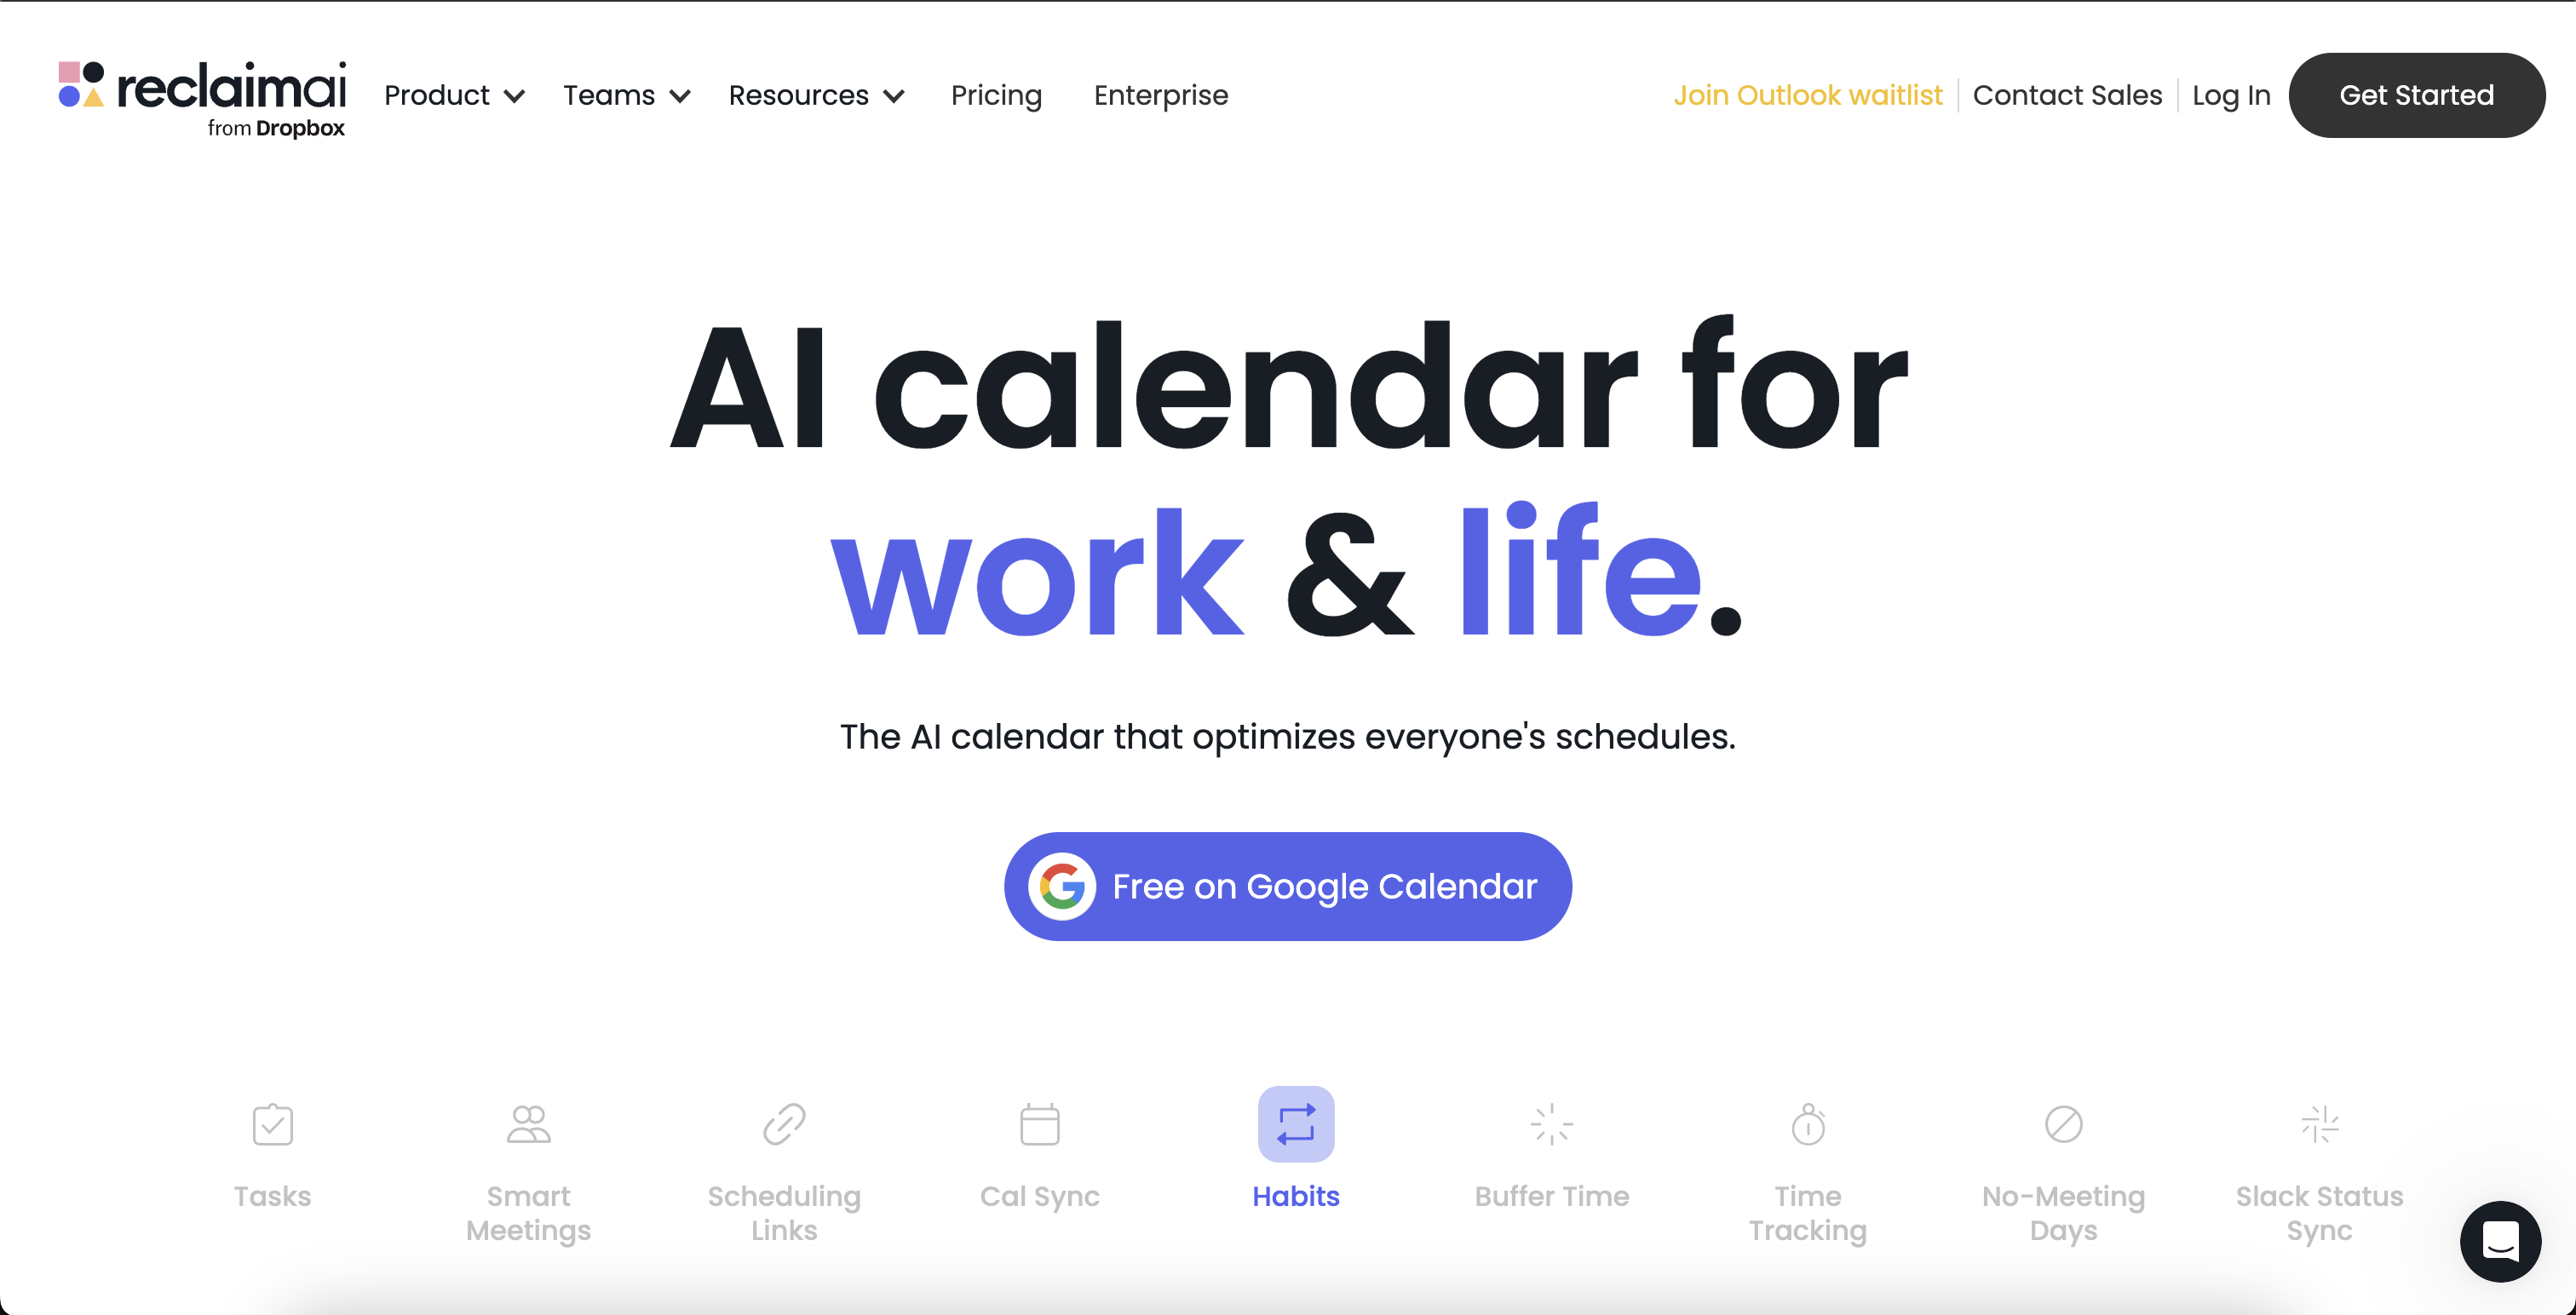
\includegraphics[width=0.8\textwidth]{images/competitors/reclaim-landing.png}
    \caption{Reclaim Landing}
    \label{fig:reclaim-landing}
\end{figure}

Reclaim.ai provides features such as smart time blocking, which automatically schedules tasks based on their priority and deadlines, integrates with tools like Google Calendar, Slack, and project management platforms (e.g., Asana, Jira, and Todoist), and supports habit tracking with auto-rescheduling to adapt to life changes. Figure~\ref{fig:reclaim-integrations} shows the integrations that this platform supports.

\begin{figure}[!h]
    \centering
    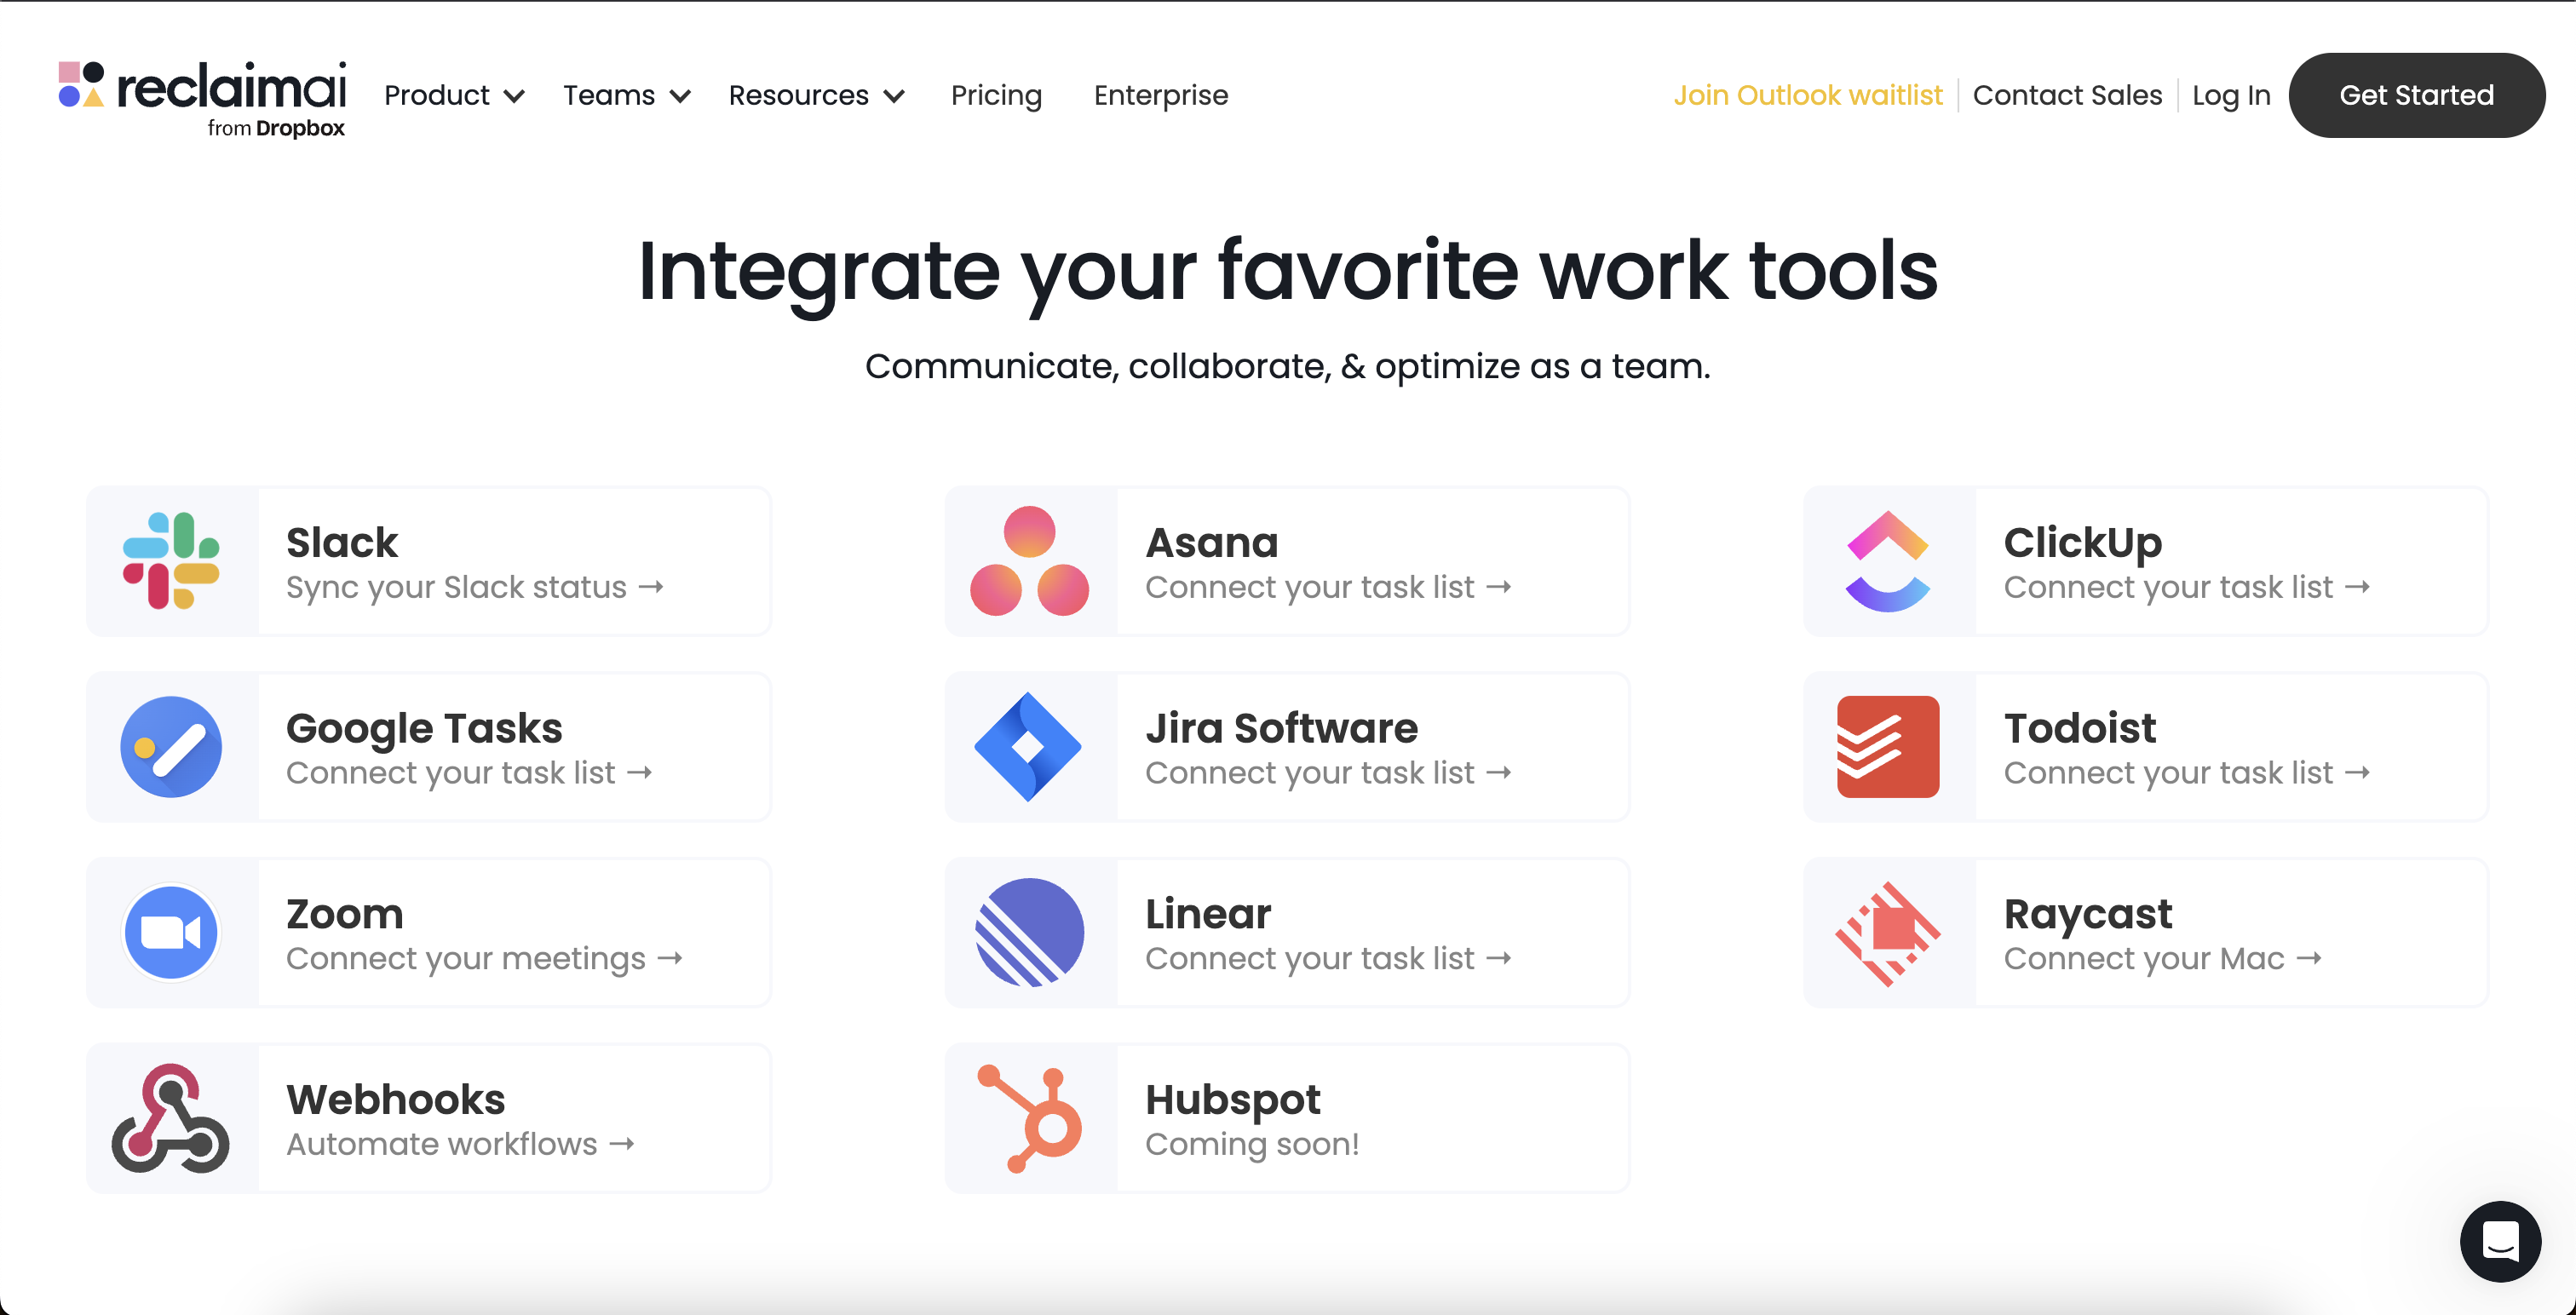
\includegraphics[width=0.8\textwidth]{images/competitors/reclaim-integrations.png}
    \caption{Reclaim Integrations}
    \label{fig:reclaim-integrations}
\end{figure}

While these features enhance productivity and optimize time management, Reclaim.ai does not include features like WhatsApp integration for automatically adding events or prayer time scheduling, both of which are unique to the Jadwal platform. These features provide users with cultural and practical benefits that further enhance their daily organization.

\subsection{Calendi}

Calendi.ai claims to offer features focused on speeding up scheduling with AI-powered assistance.

It claims to allow users to add tasks via text or voice input and automates meetings scheduling, including sending links and calendar invites.
Those claims are shown in Figure~\ref{fig:calendi-feature-voice-input}.

\begin{figure}[!h]
    \centering
    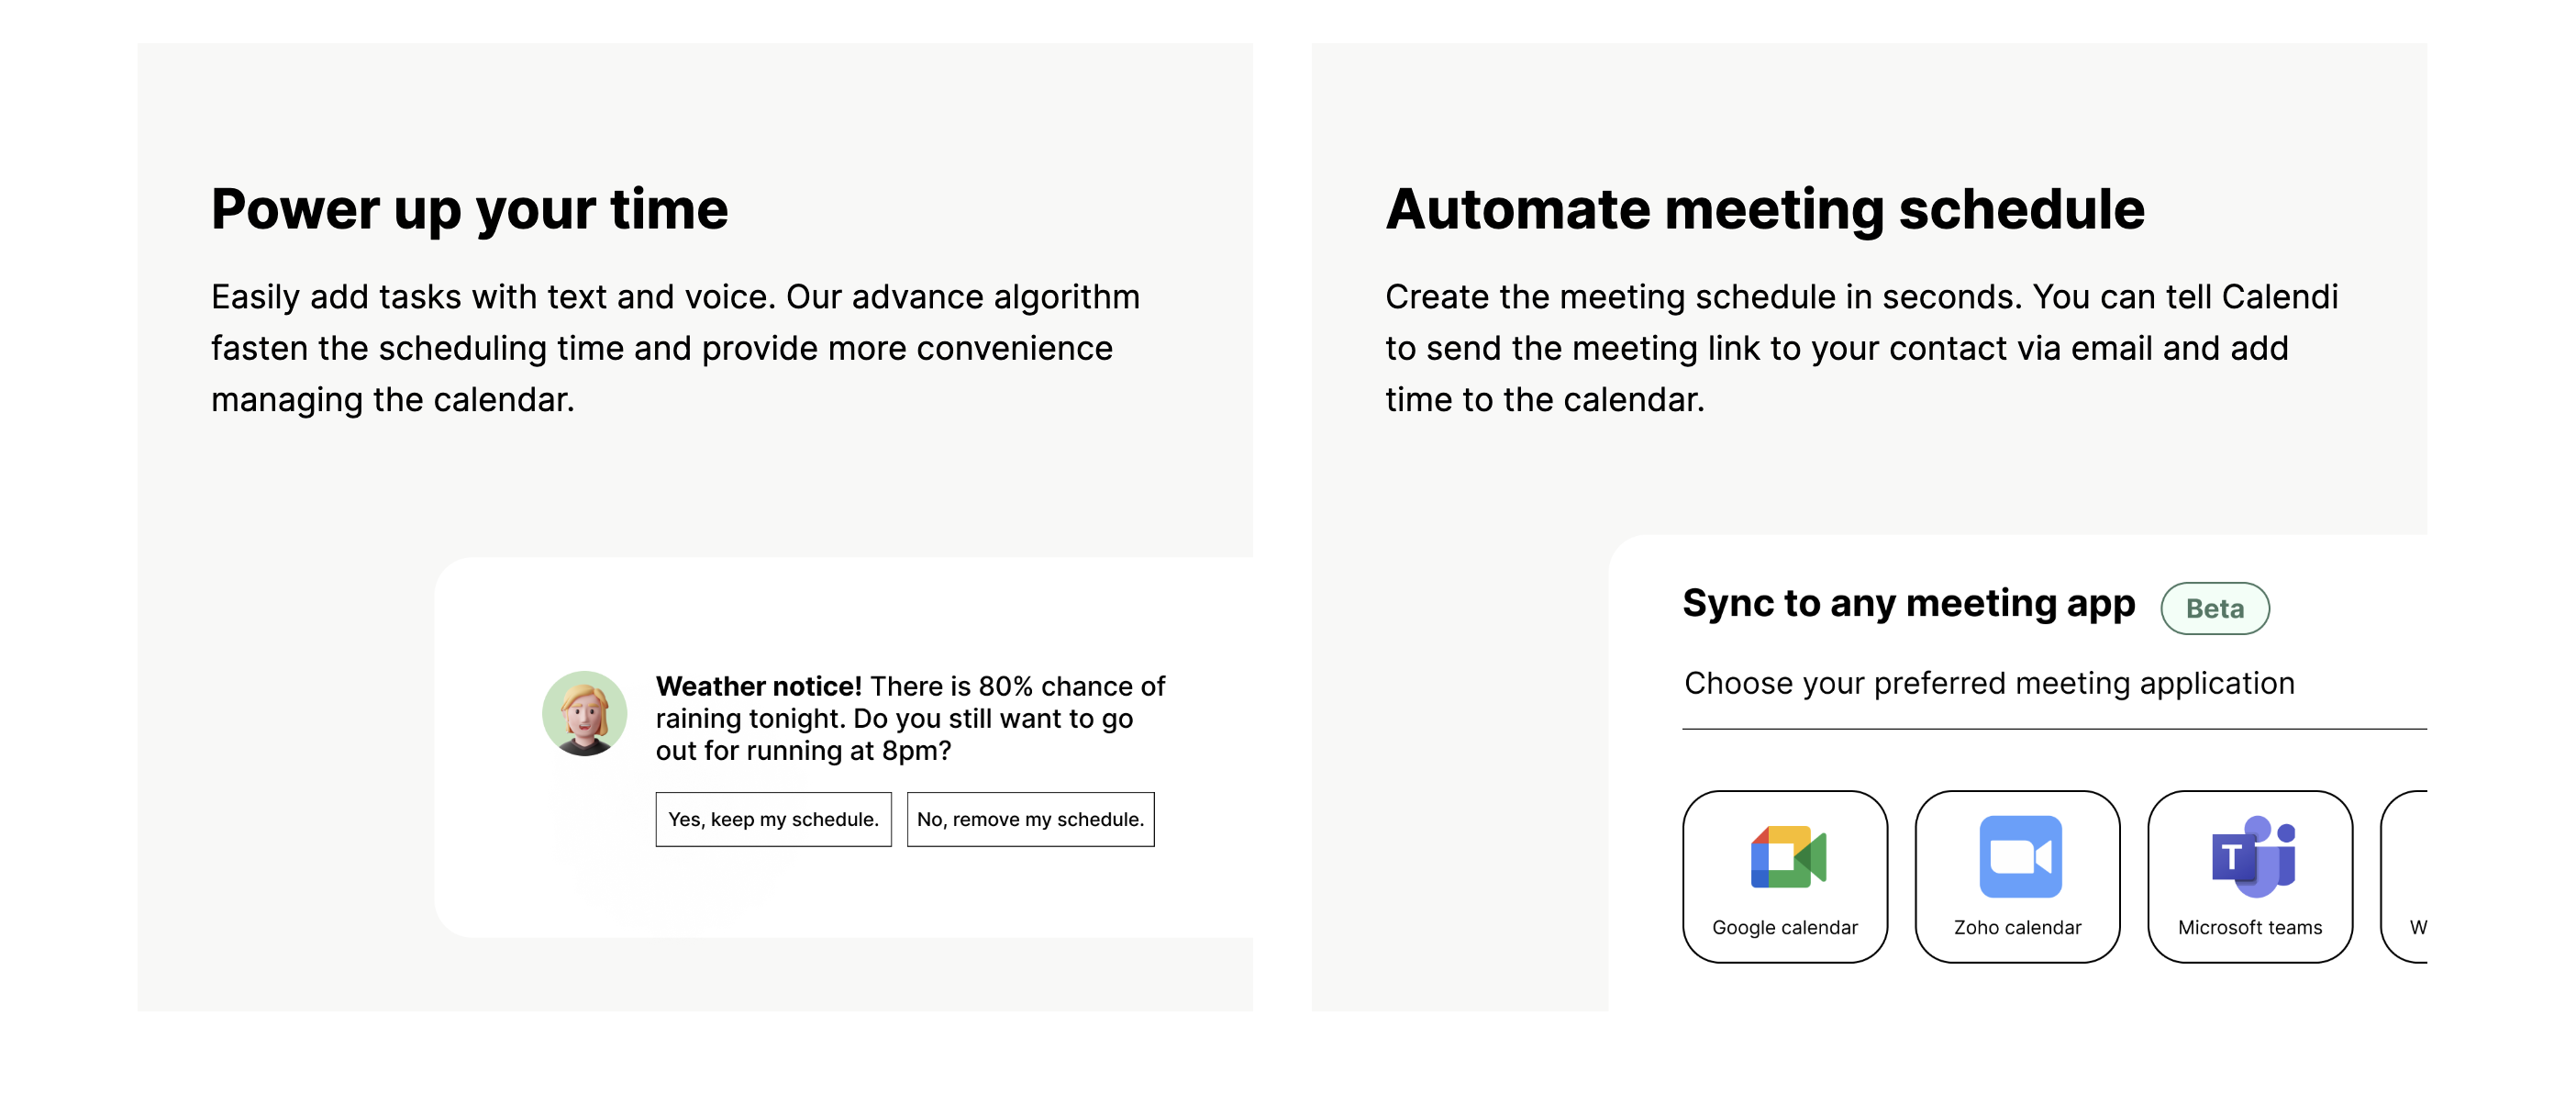
\includegraphics[width=0.8\textwidth]{images/competitors/calendi-feature-voice-input.png}
    \caption{Calendi Features of Voice Input and Automatic Meeting}
    \label{fig:calendi-feature-voice-input}
\end{figure}

Calendi claims to integrate with platforms like Google Calendar, Apple Calendar, and Outlook, making it compatible across multiple systems.
This is shown in Figure~\ref{fig:calendi-replace-em}, as they say ``We replace them all, help you save `clock emoji' `money emoji' and schedule better.''

\begin{figure}[!h]
    \centering
    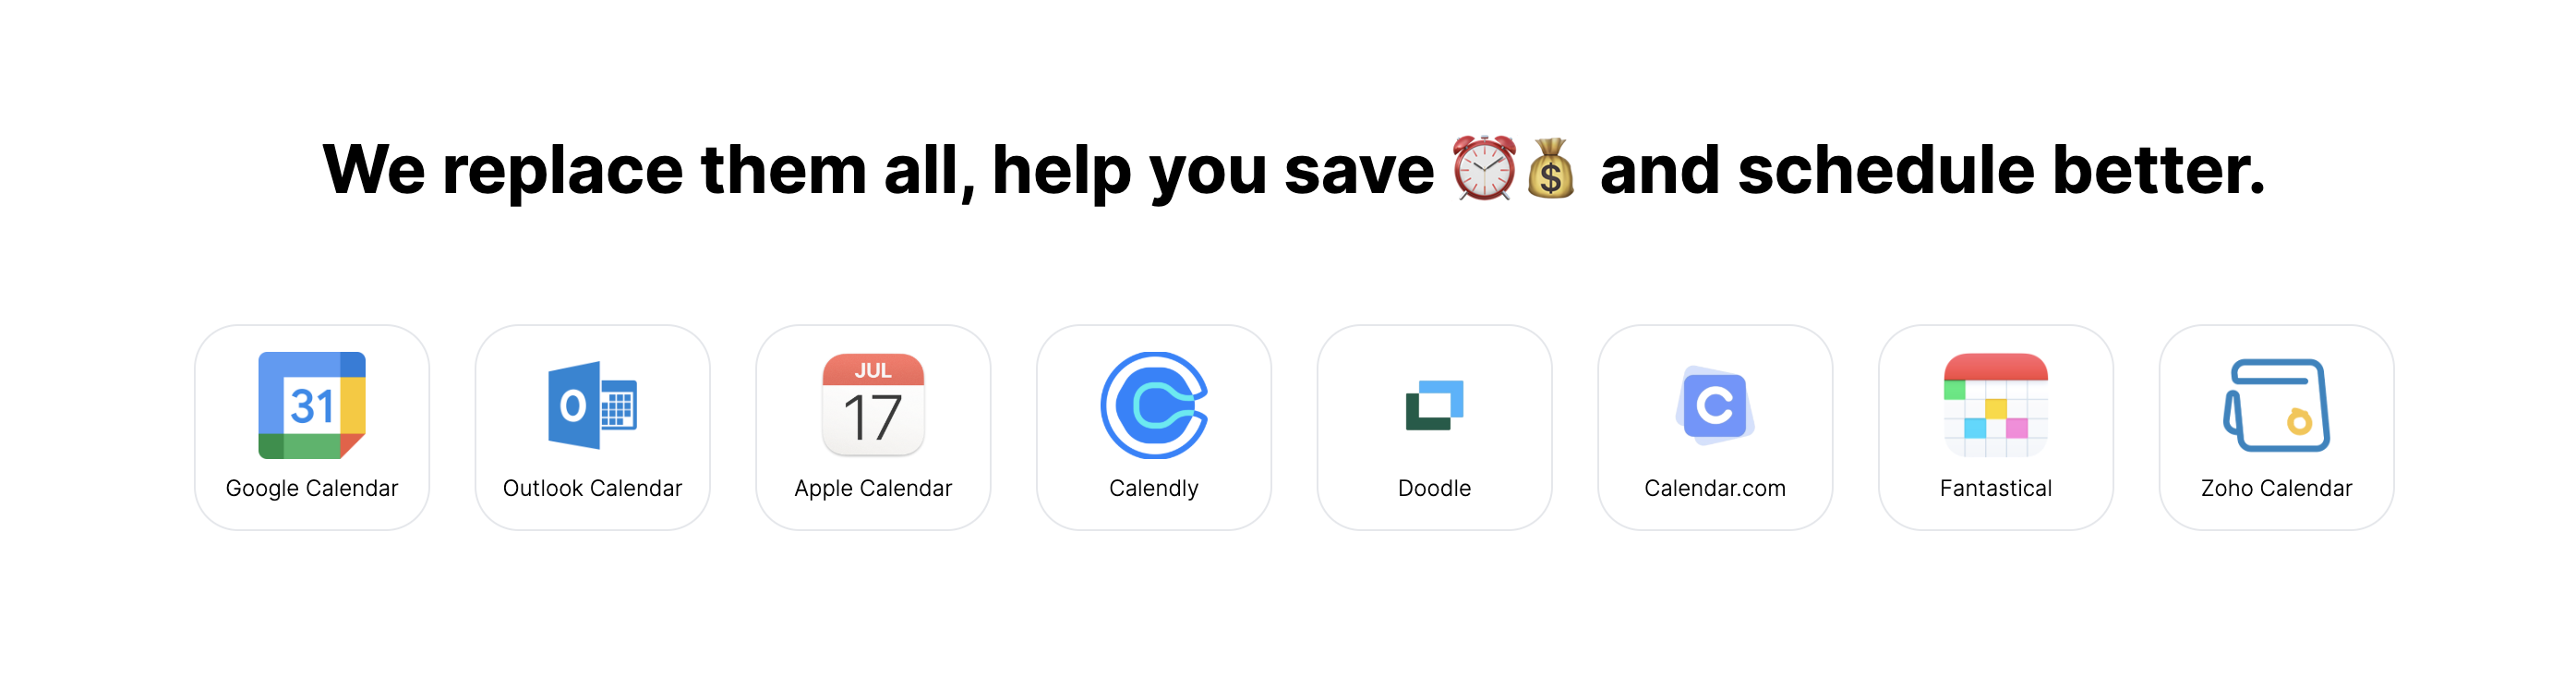
\includegraphics[width=0.8\textwidth]{images/competitors/calendi-replace-em.png}
    \caption{Calendi Claims to Replace Them All}
    \label{fig:calendi-replace-em}
\end{figure}

It claims to provide intelligent assistance by analyzing habits and tasks, suggesting improvements, and incorporating external factors like weather or transit schedules. Those are shown in Figure~\ref{fig:calendi-features}.

\begin{figure}[!h]
    \centering
    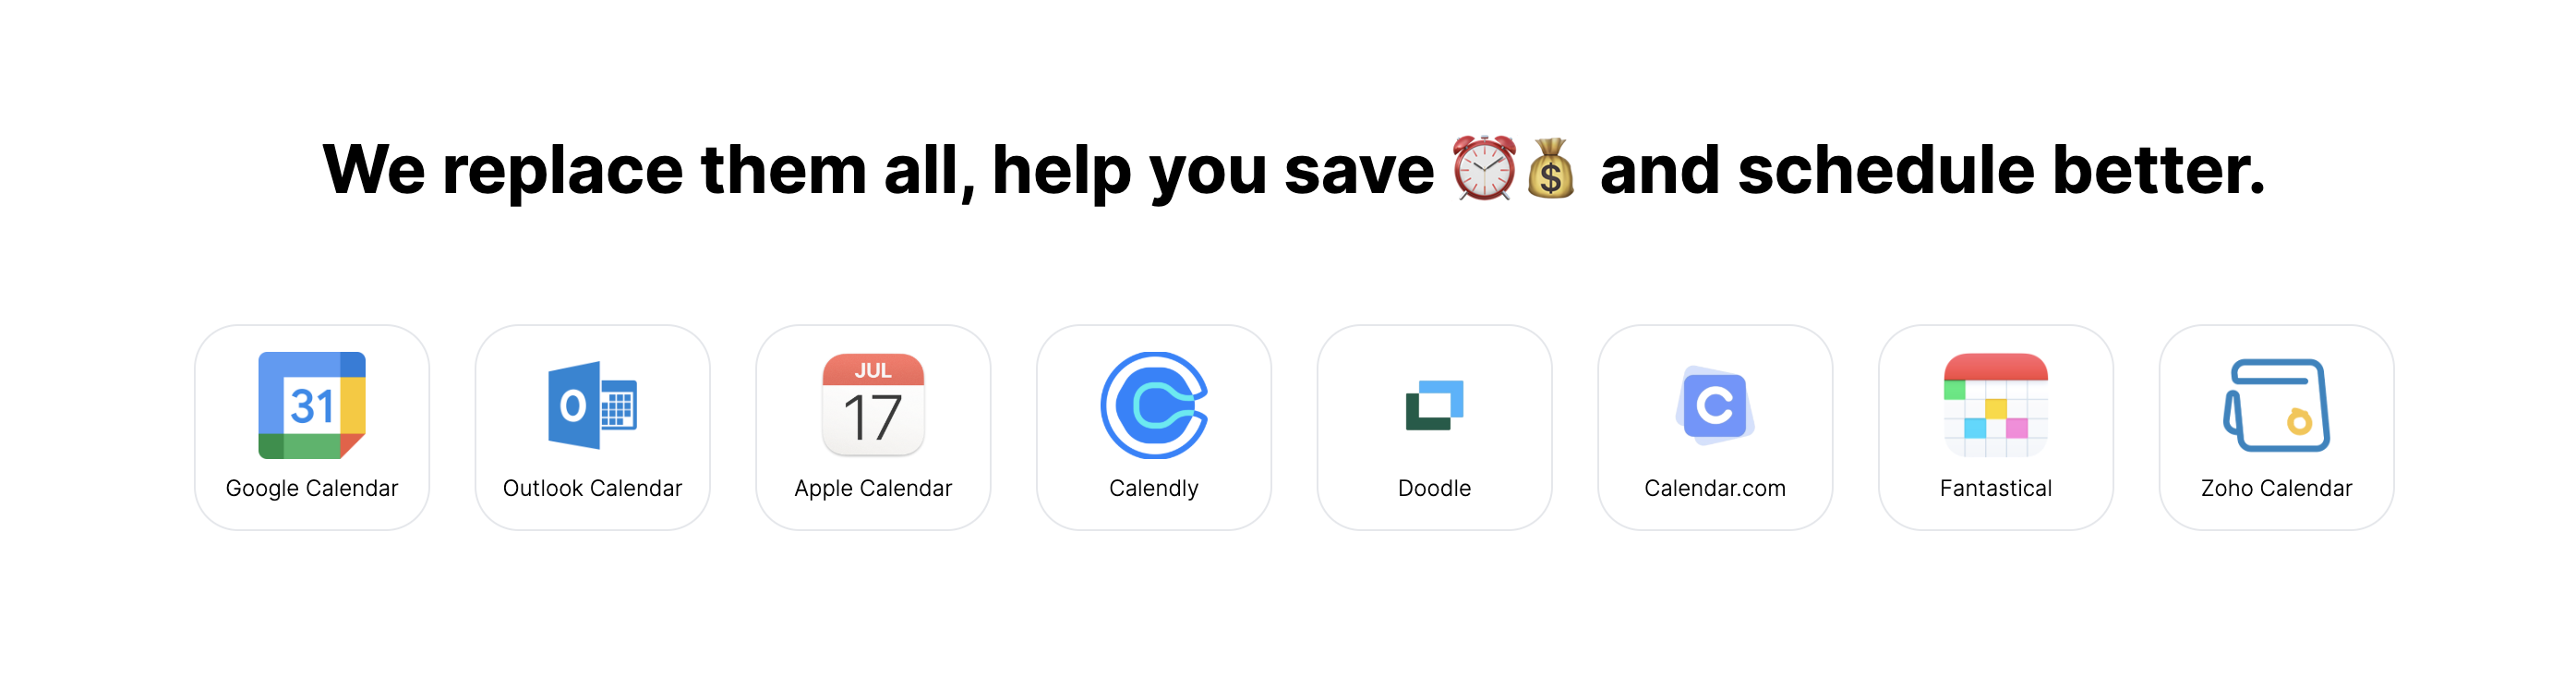
\includegraphics[width=0.8\textwidth]{images/competitors/calendi-replace-em.png}
    \caption{Calendi Claims to Replace Them All}
    \label{fig:calendi-features}
\end{figure}

However, it does not offer unique features like WhatsApp integration or prayer time scheduling, which are distinct to Jadwal.

Also the website as of writing this part, on 26 Nov 2024, is broken and not working. This can be illustrated via the broken timer shown in Figure~\ref{fig:calendi-broken-timer} and many other things that are broken.

\begin{figure}[!h]
    \centering
    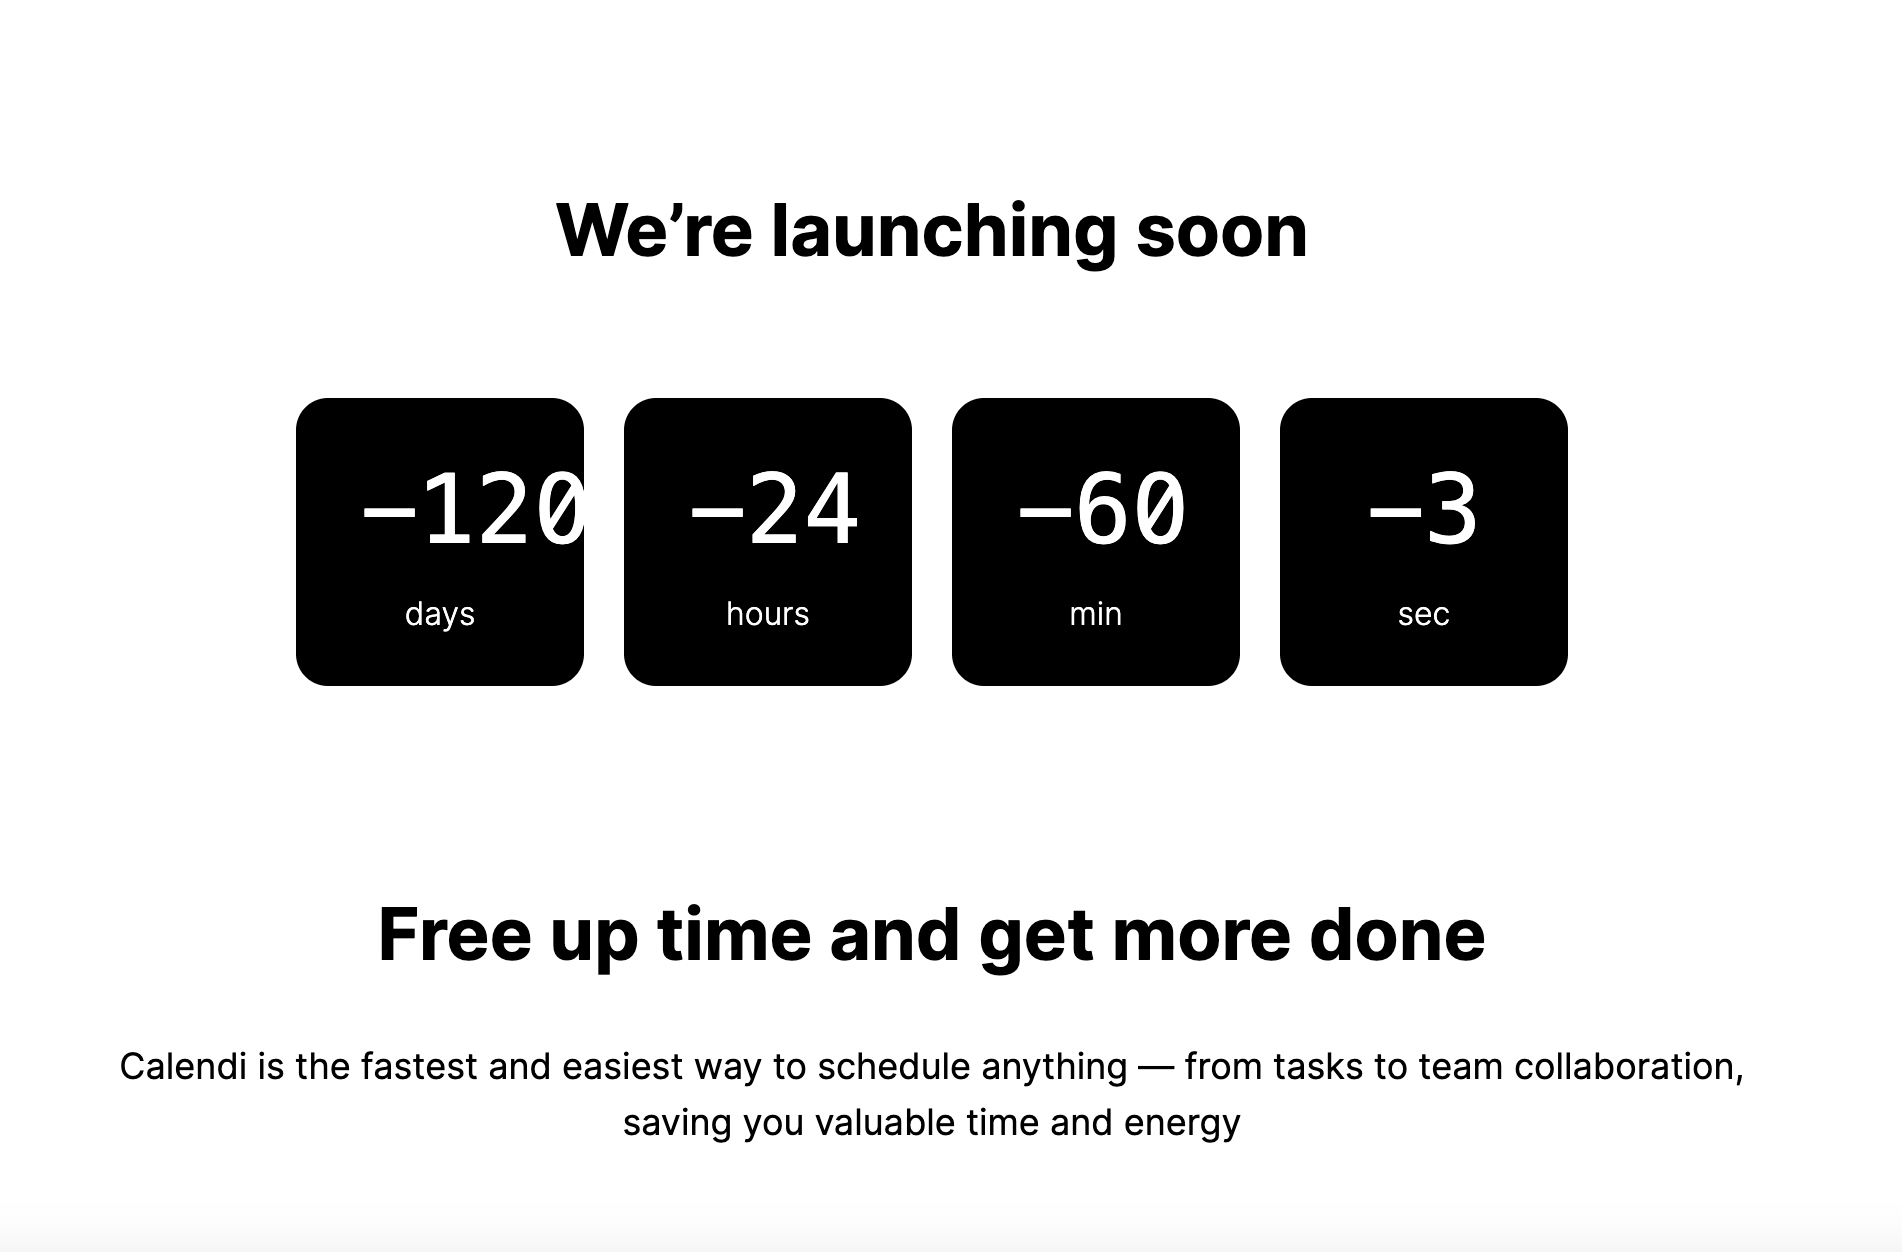
\includegraphics[width=0.8\textwidth]{images/competitors/calendi-broken-timer.png}
    \caption{Calendi Broken Timer}
    \label{fig:calendi-broken-timer}
\end{figure}

\section{Survey Results}

We have conducted a survey using Google Forms, and have sent it out to our peers in the university, and also shared it on our social media, especially LinkedIn, to get more diverse responses. That is since our main audiences are students, employees, and who do both at the same time. The results were fascinating. Especially since 75 responses were recorded with their email to authenticate the responses.

As shown in Figure~\ref{fig:survey-status}, the results showed that 8\% only were both employed and students, while 53\% were students only and 39\% were employed only. We believe this is a good mix between the two audience we are aiming to get responses from.

\begin{figure}[!h]
    \centering
    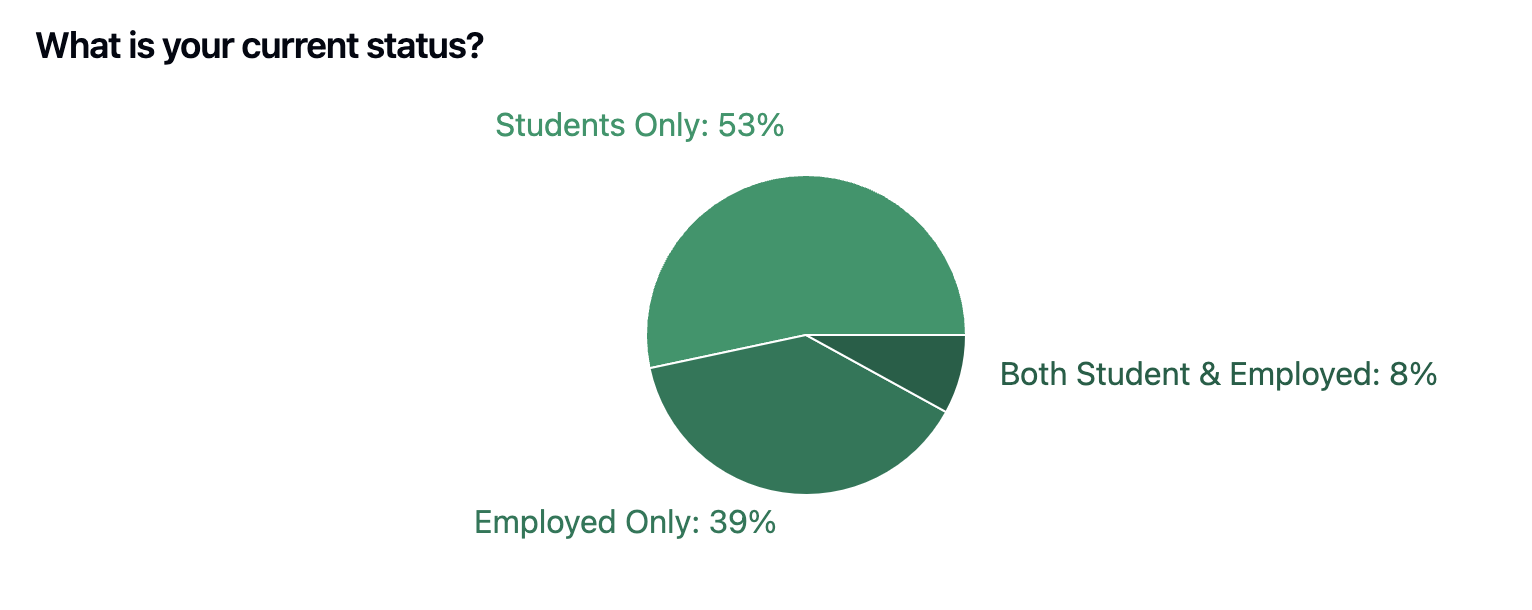
\includegraphics[width=0.8\textwidth]{images/survey/status.png}
    \caption{Survey Respondents Status}
    \label{fig:survey-status}
\end{figure}

Based on Figure~\ref{fig:age-range}, it is important to note that 72\% of our respondents were of the age range 20-30 years.

\begin{figure}[!h]
    \centering
    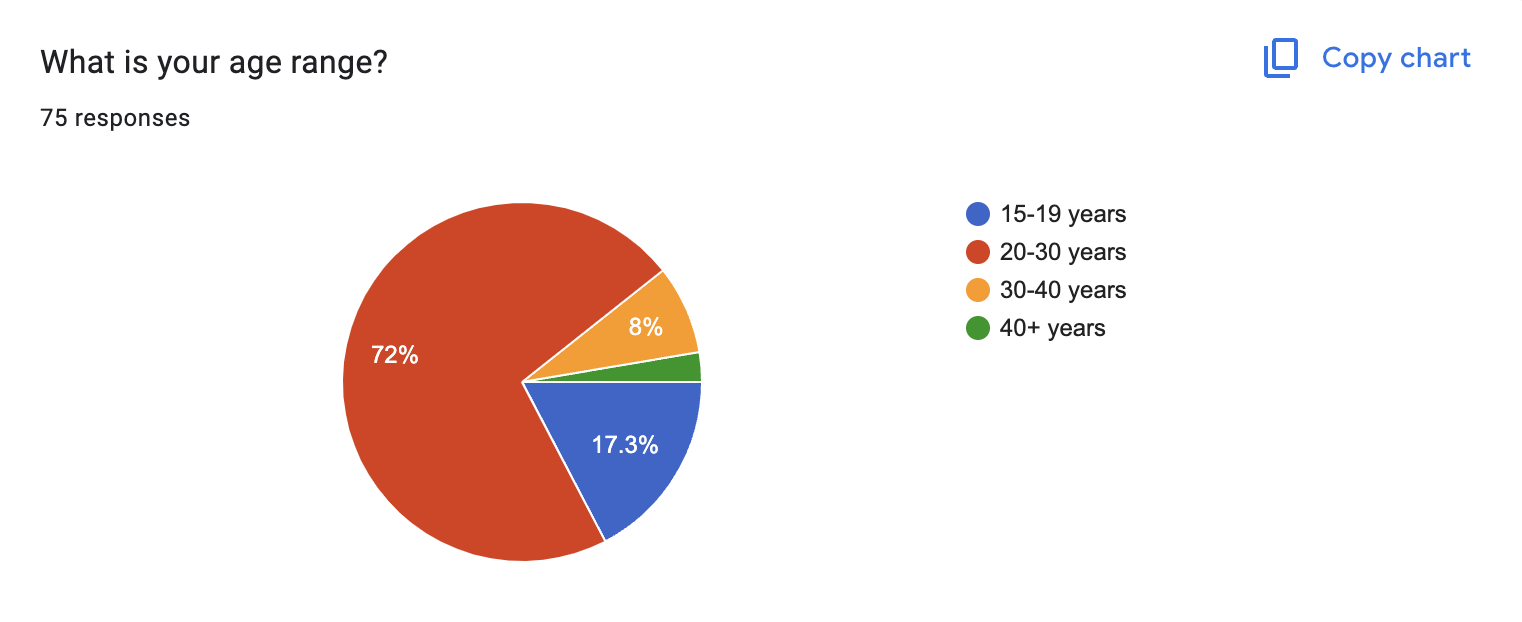
\includegraphics[width=0.8\textwidth]{images/survey/age.png}
    \caption{Age Range}
    \label{fig:age-range}
\end{figure}

As shown in Figure~\ref{fig:use-calendar}, 66.7\% of people reported that they a calendar application to manage their daily schedule. This shows that people might be interested in a better way of managing their schedules that could elevate their time management skills.

\begin{figure}[!h]
    \centering
    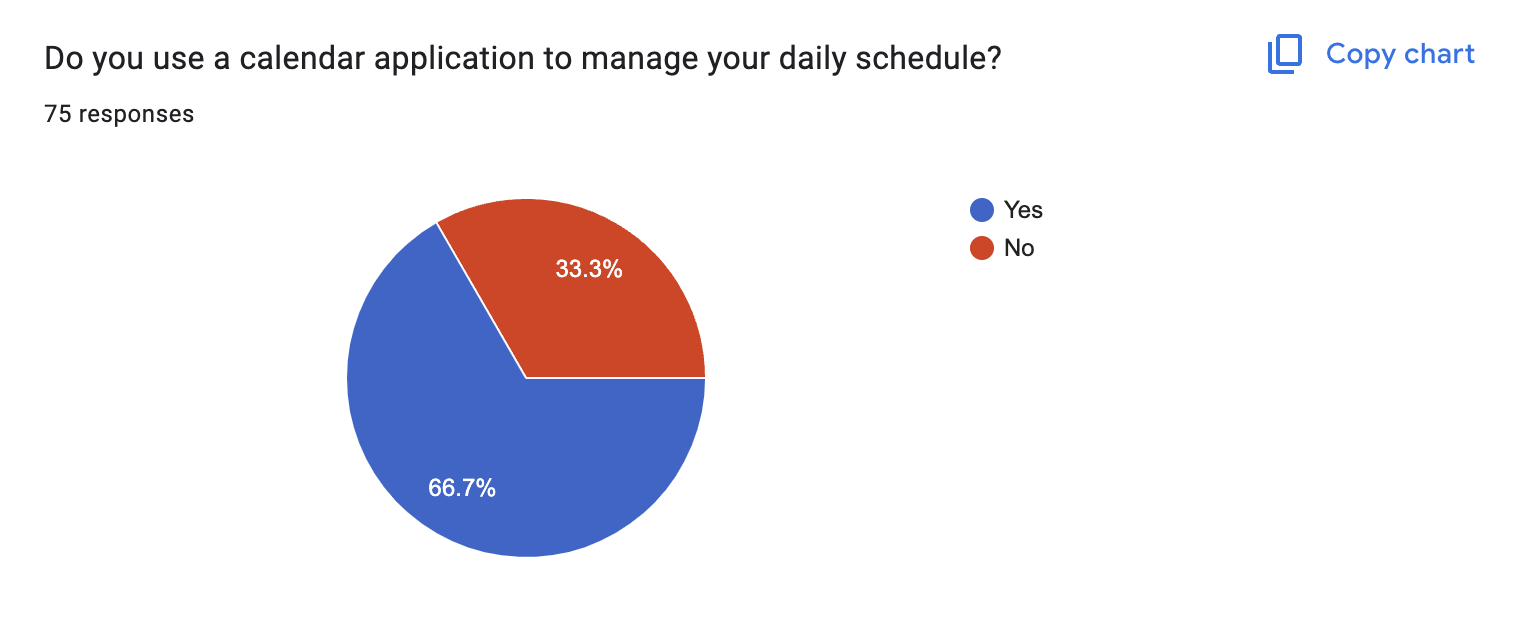
\includegraphics[width=0.8\textwidth]{images/survey/use-calendar.png}
    \caption{Percentage of People Who Use Calendars to Ones Who Don't}
    \label{fig:use-calendar}
\end{figure}

In Figure~\ref{fig:platform-to-discuss}, the results showed us the need for our app to exist, since 70.7\% of the population use WhatsApp to discuss upcoming events! Another big percentage, 53.3\% used Email also. Our app won't be focusing on this, nevertheless, this is also an opportunity in the future to help those people who use Emails and might not find the flow easy to schedule the events in the calendar.

\begin{figure}[!h]
    \centering
    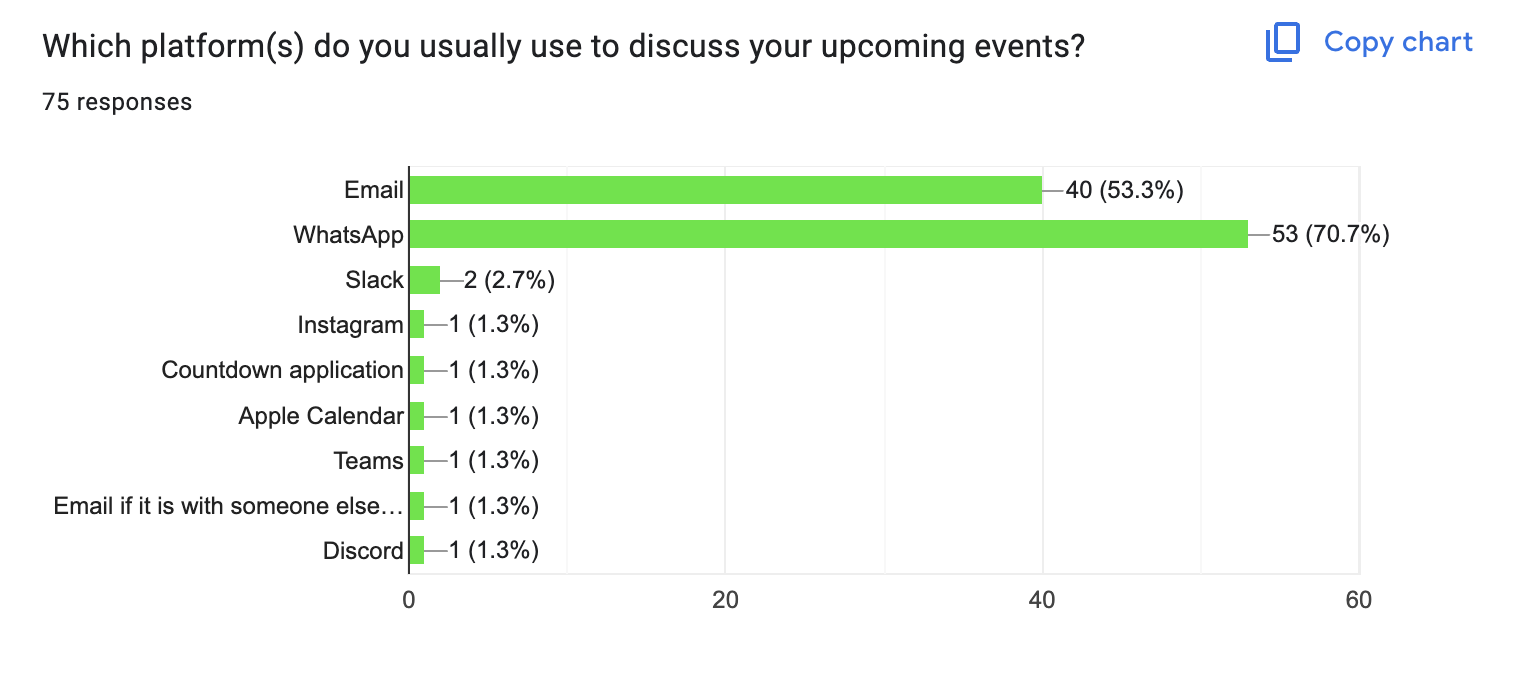
\includegraphics[width=0.8\textwidth]{images/survey/platform-to-discuss.png}
    \caption{Platform Used to Discuss}
    \label{fig:platform-to-discuss}
\end{figure}

Although 21.3\% might not seem like a lot, but as shown in Figure~\ref{fig:usefullness}, 58.7\% of the population reported they would find it extremely useful to have a WhatsApp integration that automatically adds events from your conversations to the calendar?

\begin{figure}[!h]
    \centering
    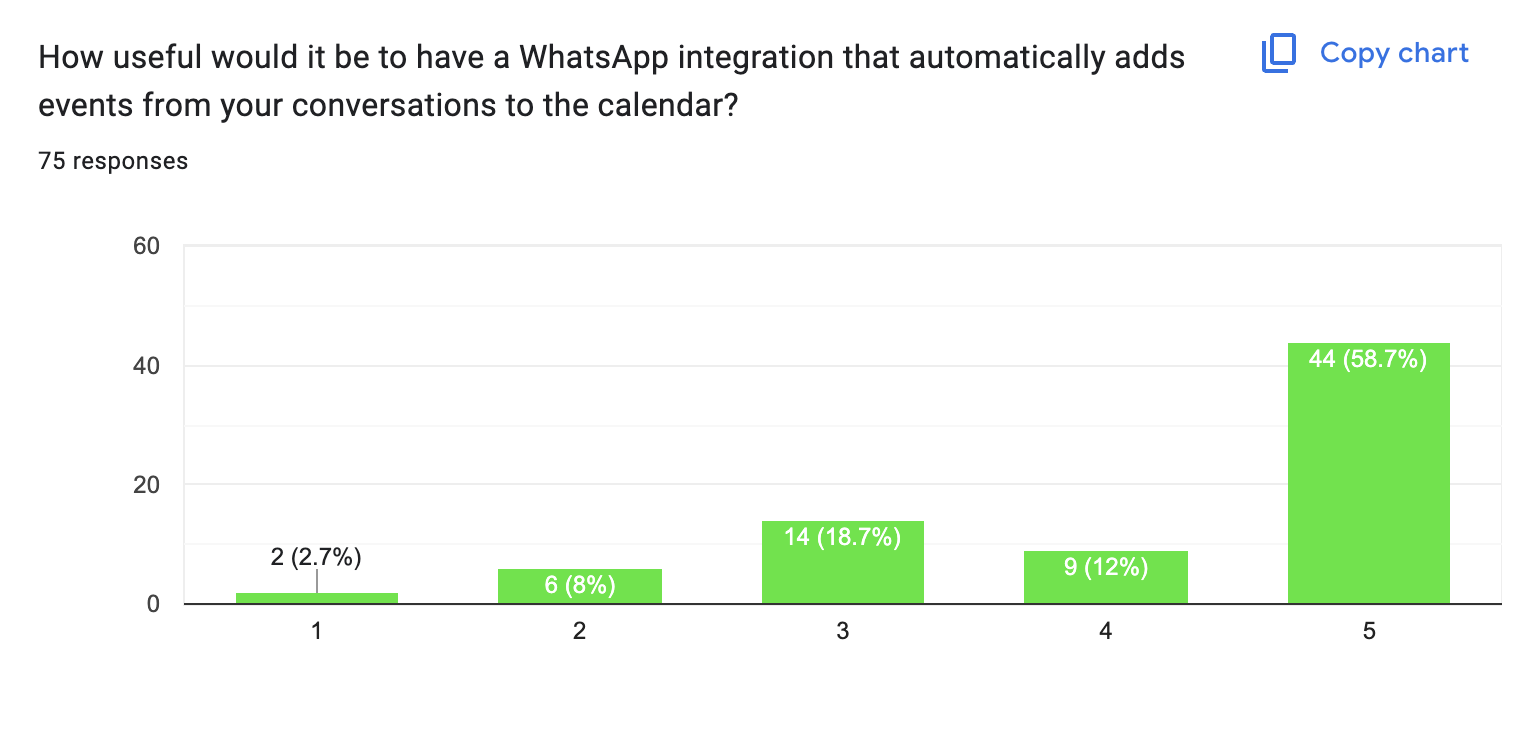
\includegraphics[width=0.8\textwidth]{images/survey/usefullness.png}
    \caption{Usefulness of Having a WhatsApp Integration}
    \label{fig:usefullness}
\end{figure}

As shown in Figure~\ref{fig:forget-to-add}, on average, 21.3\% forget to add events to their calendar. That is great news, since our differentiating factor is the direct WhatsApp integration that should be able to solve this.

\begin{figure}[!h]
    \centering
    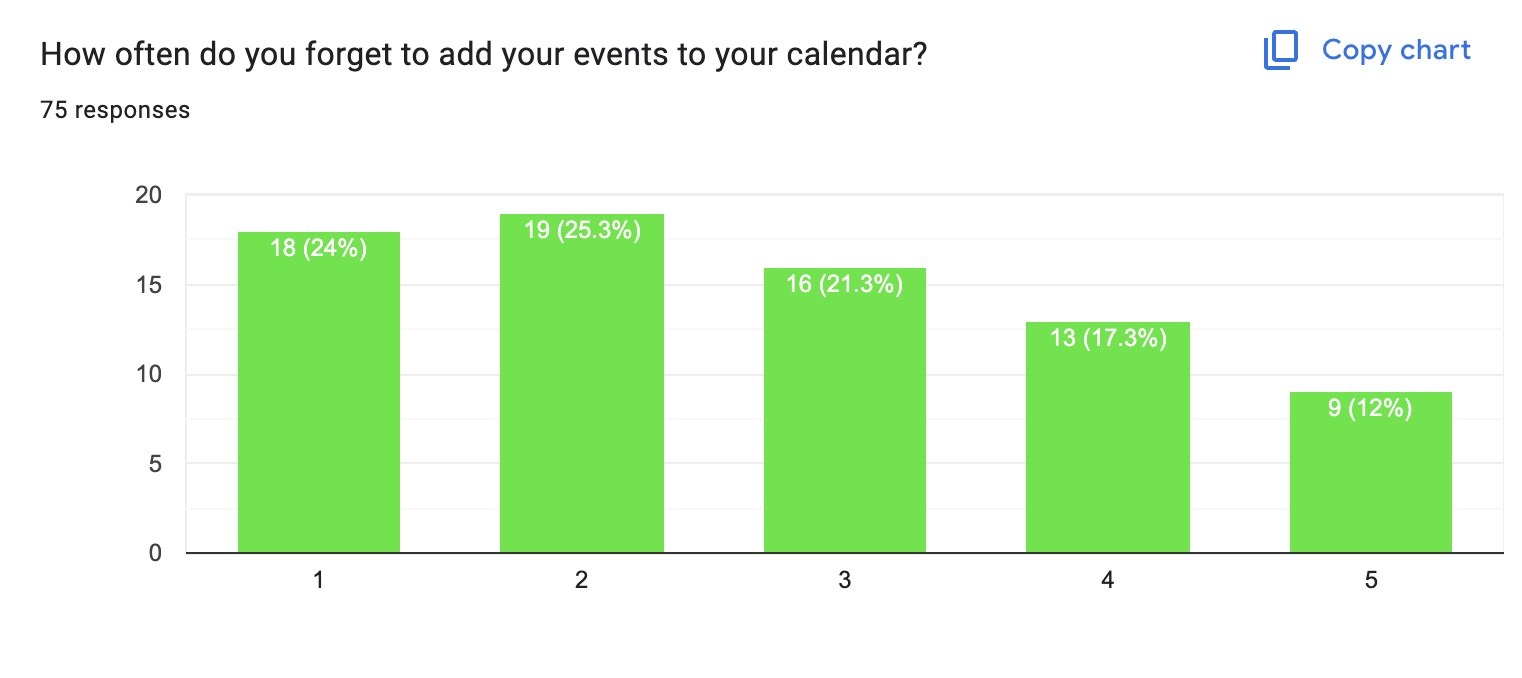
\includegraphics[width=0.8\textwidth]{images/survey/forget-to-add.png}
    \caption{Chart of Forgetting to Add Likeliness}
    \label{fig:forget-to-add}
\end{figure}

As shown in Figure~\ref{fig:number-of-calendars}, 41.3\% use 2 calendars, that shows the need for a integrated view of calendars.

\begin{figure}[!h]
    \centering
    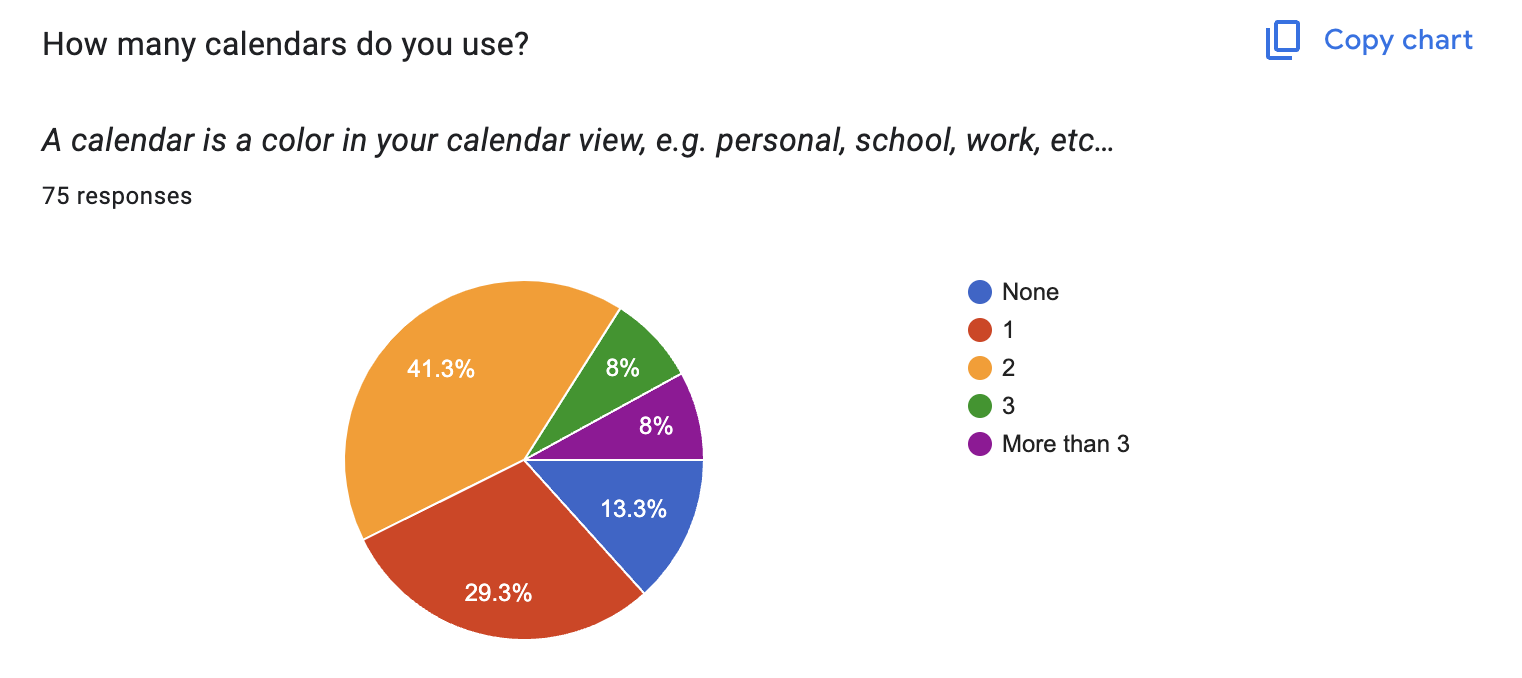
\includegraphics[width=0.8\textwidth]{images/survey/number-of-calendars.png}
    \caption{Number of Calendars}
    \label{fig:number-of-calendars}
\end{figure}

As shown in Figure~\ref{fig:events-per-week}, 53.3\% of people have 1-3 calendar events per week. That might seem a little, but 33.3\% have 4-6 calendar events per week.

\begin{figure}[!h]
    \centering
    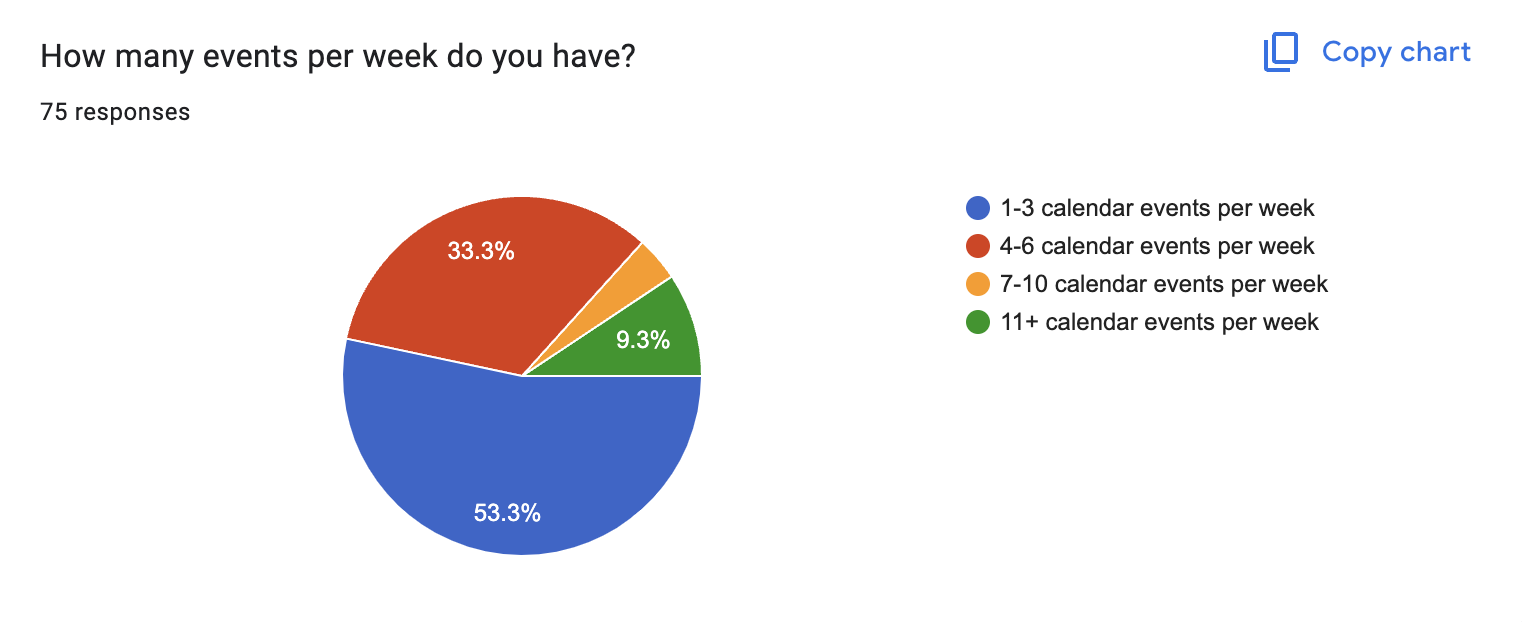
\includegraphics[width=0.8\textwidth]{images/survey/events-per-week.png}
    \caption{Events per Week}
    \label{fig:events-per-week}
\end{figure}

\section{Conclusion}

Through this literature review, we have identified several key gaps in existing calendar management solutions. While platforms like Clockwise, Motion, Reclaim AI, and Calendi have made significant strides in intelligent scheduling and calendar integration, none provide a comprehensive solution that addresses the full spectrum of modern scheduling challenges. The review reveals three primary opportunities for innovation:

First, while existing solutions focus on traditional calendar management, there remains an untapped potential in integrating informal communication channels. Jadwal's WhatsApp integration addresses this gap, offering automated event extraction from everyday conversations—a feature notably absent in current market offerings.

Second, our analysis shows that while many applications offer conflict resolution features, none combine this with prayer time prioritization, creating a unique opportunity to serve users who prioritize religious obligations alongside professional commitments.

Finally, the review demonstrates that current solutions often operate in isolation, whereas Jadwal's approach of unifying multiple calendars while maintaining intelligent event extraction and conflict resolution presents a more holistic solution to modern scheduling challenges.

These findings validate Jadwal's approach and highlight its potential to address significant unmet needs in the calendar management space, particularly in combining automation, religious considerations, and comprehensive calendar integration.

\cleardoublepage
